The Precision Timed ARM (PTARM) architecture is a realization of the PRET principles on an ARM instruction set architecture\todo{Citation}. 
In this chapter we will describe in detail the implementation of the timing-predictable ARM processor and discuss the worst-case execution time analysis of code running on it.
We show that with the architectural design principles of PRET, the PTARM architecture is easy analyzable with repeatable timing.
  
The architecture of PTARM closely follows the principles discussed in chapter~\ref{chapter:pret}.
This includes a thread-interleaved pipeline with scratchpads along with the timing predictable memory controller.
The ARM ISA was chosen not only for its popularity in the embedded community, but also because it is a Reduced Instruction Set Computer (RISC), which has simpler instructions that allow more precise timing analysis. 
Complex Instruction Set Computers (CSIC) on the other hand adds un-needed complexity to the hardware and timing analysis.
RISC architectures typically features a large uniform register file, a load/store architecture, and fixed-length instructions.
In addition to these, ARM also contains several unique features.
ARM's ISA requires a built in hardware shifter along with the arithmetic logic unit (ALU), as all of its data-processing instructions can shift its operands before passed onto the ALU. 
ARM's load/store instructions also contain auto-increment capabilities that can increment or decrement the value stored in the base address register. 
This is useful to compact code that is reading through an array in a loop, as one instruction can load the contents and prepare for the next load in one instruction.
In addition, almost all of the ARM instructions are conditionally executed.
The conditional execution improves architecture throughput with potential added benefits of code compaction\todo{Citation}.     
ARM programmer's model specifies 16 general purpose registers (R0 to R15) to be accessed with its instructions, with register 15 being the program counter (PC). 
Writing to R15 triggers a branch, and reading from R15 reads the current PC plus 8.

ARM has a rich history of versions for their ISA, and PTARM implements the ARMv4 ISA, currently without support for the thumb mode.
PTARM uses scratchpads instead of caches, and a DDR2 DRAM for main memory managed by the timing predictable memory controller.
PTARM also implements the timing instructions introduced in chapter~\ref{sec:programming_models}.   
%We will first discuss the architectural details of PTARM, then present the C++ software simulator.   

\section{Thread-Interleaved Pipeline}
PTARM implements a thread-interleaved pipeline for the ARM instruction set.
PTARM was initially written to target Xilinx Virtex-5 Family FPGAs, thus several design decisions were made to optimized the PTARM architecture for Xilinx V5 FPGAs.
PTARM has a 32 bit datapath in a five stage pipeline with four threads interleaving through the pipeline. 
Chapter~\ref{chapter:pret} discussed the timing and hardware benefits of a typical thread-interleaved pipeline which removes pipeline hazards with multiple threads.
Section~\ref{section:pret_thread_pipeline} mentioned that conventional thread-interleaved pipelines typically have at least as many threads as pipeline stages to keep the pipeline design simple and maximize the clock speed.
However, having more threads in the pipeline increases single thread latency, since all threads are essentially time-sharing the pipeline resource. 
Lee and Messerschmitt~\cite{lee1987pip} showed that the minimum number of threads required to remove hazards is actually less than the number of pipeline stages in the pipeline. 
In our design, we implement a five stage thread-interleaved pipeline with four threads by carefully designing the PC writeback mechanism one pipeline stage earlier.

Figure~\ref{fig:ptarm_pipeline_five_stage} shows a block diagram view of the pipeline. 
Some multiplexers within the pipeline have been omitted in the figure for a simplified view of the hardware components that make up the pipeline.
There contains four copies of the Program Counter(PC), Thread States, and Register File.
Most of the pipeline design follows a typical Hennessy and Patterson\todo{citation} five stage pipeline, with the five stages in the pipeline being -- Fetch, Decode, Execute, Memory, Writeback.
We will briefly describe the functionality of each stage, and leave more details when we discuss how instructions are implemented in section~\ref{sec:ptarm_instructions}.

\begin{figure}[b]
  \vspace{-20pt}
  \begin{center}
    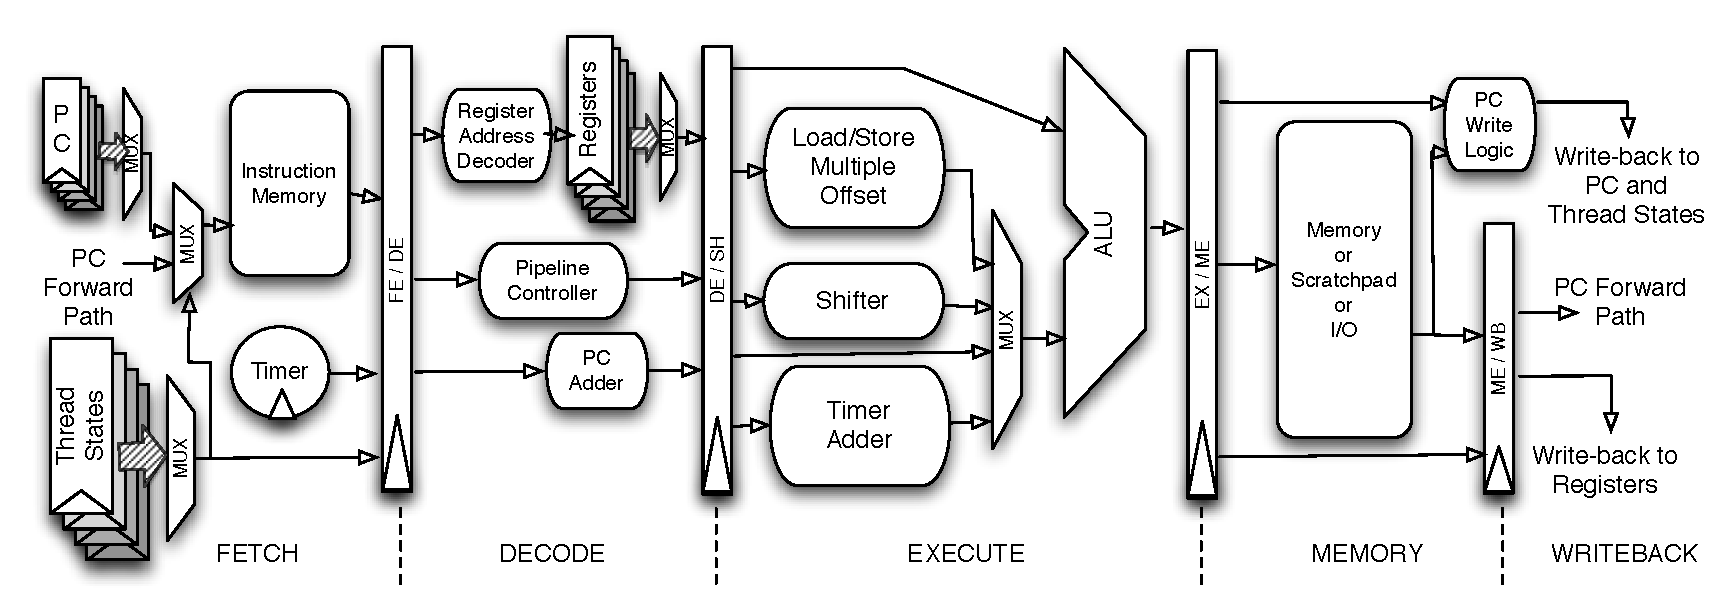
\includegraphics[scale=.54]{figs/ptarm_pipeline_five_stage}
  \end{center}
  \vspace{-20pt}
  \caption{Block Level View of the PTARM 5 stage pipeline}
  \label{fig:ptarm_pipeline_five_stage}
\end{figure}

%The \emph{fetch} and \emph{decode} stages setup the data operands and control signals for the later stages to execute the instruction.
The \emph{fetch stage} of the pipeline selects the correct PC according to which thread is executing, and passes the address to instruction memory. 
The PC forward path forwards a loaded address from main memory for instructions that load to R15, which causes a branch.
We will discuss the need for the forwarding path below when we describe the \emph{writeback stage}.
A simple $log(n)$ bit upcounter is used to keep track of which thread current to fetch.

The \emph{decode stage} contains the \emph{pipeline controller} which does the full decoding of instructions and sets the correct pipeline signals to be propagated down the pipeline.
Most of ARM instructions are conditionally executed, so the pipeline controller first checks the condition bis to determine whether the instruction is to be executed or not.  
Typically the \emph{pipeline controller} needs to know the current instructions in the pipeline to detect the possibility of pipeline hazards and stall the current instruction.
However,in a thread-interleaved pipeline, other instructions down the pipeline are from threads, thus the controller logic is greatly simplified. 
It simply decodes the instruction to determine the correct signals to send to the data-path and multiplexers down the pipeline.
It does not need to know any information about instructions already in flight. 
A small decoding logic, the \emph{register address decoder}, is inserted in parallel with the controller to decode the register addresses from the instruction bits.  
Typical RISC instruction sets, such as MIPS, set the encoding of instruction bits so the register operands have a fixed location for all instruction types.
However, in the ARM instruction set, certain instructions encode the register read address at different bit locations of the instruction.
For example, ARM data-processing register shift instructions reads a third operand from the register to determine the shift amount.
Store instructions also read a third register to obtain the register value that is stored to memory. 
However, both instructions have different bit locations in the instruction encoding to determine what register to read from.
Thus, a small register address decoding logic is inserted for a quick decoding of the register addresses from the instruction bits.
The \emph{PC Adder} is used to increment the PC.
%FIXME: Talk about the design of the ISA to optimize pipeline implementation, which in our case did not make things easier
The ARM ISA programmer's model states that reading from R15 reads the current PC+8, the PC adder not only increments the PC by 4 to get the potential next PC, but it also increments the current PC by 8 to be used as an operand. 
Single threaded pipelines need to increment the PC immediately in the fetch stage to prepare for the next instruction fetch.  
For thread-interleaved pipelines, since the next PC from the current thread is not needed until several cycles later, it doesn't need to be in the fetch stage. 
But because we need the results of PC+8 as a data operand, it is placed in the decode stage. 
The \emph{timer} is a hardware counter clocked to the processor clock which is used to implement the timing instructions mentioned in section~\ref{sec:programming_models}.
The timer contains a 64 bit value that represents nanoseconds, and starts at 0 when the pipeline starts up.  
The time value is latched in the decode stage as the subsequent stages use it for timer manipulation.

The \emph{execute}, \emph{memory} and \emph{writeback} stages execute the instruction and commits the result. 
The \emph{execute} stage contains mostly execution units and muxes that select the correct operand and feeds it to the ALU.  
The ARM ISA assumes a built in shifter to shift the operands before operations, so a 32 bit \emph{shifter} is included to shift the operands before the ALU.   
The \emph{load/store multiple offset} logic block is used to calculate the offset of load/store multiple instructions.
The load/store multiple instruction uses a 16 bit vector to represent each of the 16 general purpose registers.
The bits that are set in that bit vector represents a load/store on that register.
The an offset is added to the base memory address for the instruction, and that offset depends on how many bits are set. 
Thus, the load/store multiple offset logic block does a bit count on the bit vector and adjusts the offset to be passed into the ALU for load/store multiple instructions.
The \emph{timer adder} logic block is a 32 bit add/subtract unit.
Time in the pipeline is a 64 bit value representing nanoseconds. 
Thus, any timing instruction that interacts with the timer in the pipeline needs to operate on 64 bit values.
We could have reuse the existing ALU at the expense of having all timing instructions take an additional pass through the pipeline.
But we chose to include an addition add/subtract unit specifically for the implementation of the delay\_until instruction so it can check for deadline expiration every cycle, which we will discuss in detail in section~\ref{sec:ptarm_instructions} when we show how delay\_until is implemented.    
A 32 bit \emph{ALU} does most of the logical and arithmetic operations, including data-processing operations and branch address calculations.
The results is passed to the \emph{memory stage}, which either uses it as an address to interact with the data memory, or forwards it along to the \emph{writeback stage} to commit back to the registers.

\begin{wrapfigure}{r}{0.5\textwidth}
  \vspace{-20pt}
  \begin{center}
    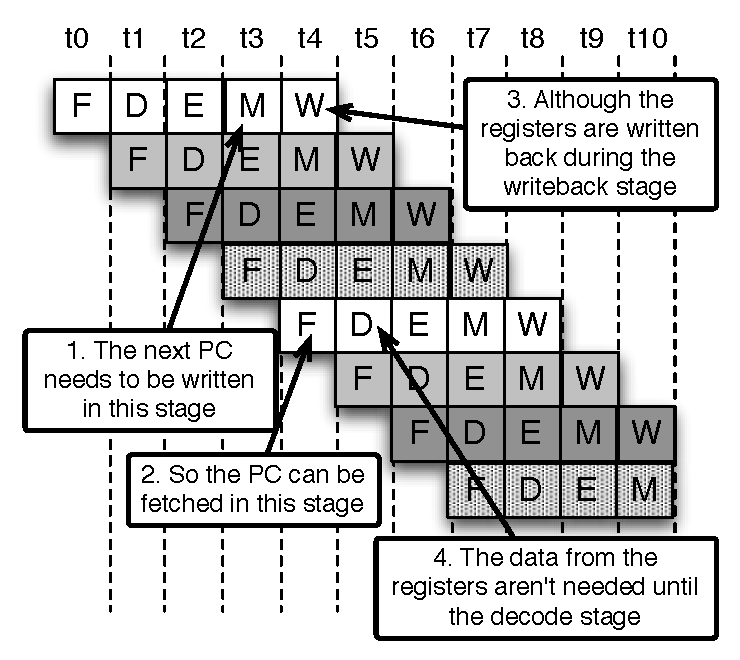
\includegraphics[scale=.65]{figs/four_thread_pipeline}
  \end{center}
  \vspace{-20pt}
  \caption{Four thread execution in PTARM}
  \label{fig:four_thread_pipeline}
  \vspace{-10pt}
\end{wrapfigure}      
%Although the register values are committed in the write back stage, the next PC address needs to be written back earlier. 
Figure~\ref{fig:four_thread_pipeline} shows an execution sequence of the four thread five stage pipeline.
The instruction in the fetch stage belongs to the same thread as the instruction in the writeback stage.
This does not cause any data hazards because the data from the registers will not be read until the decode stage. 
But committing the PC at the writeback stage would result in a control hazard because the PC would not be ready for the subsequent fetch.
For most instructions, the next PC calculation is completed before the memory stage, so we move the PC commit one stage earlier so the next instruction can be fetched.
However, the ARM ISA allows instructions to write to register 15 (PC), which acts as a branch to the value written to R15.   
This means a load instruction can write to R15 and cause a branch whose target is not known until after the memory read.   
Thus, a PC forwarding path is added to forward the PC back from memory if a load instruction writes to R15.  
The forwarding path does not cause any timing analysis difficulties because the statically the forwarding path is only used when a load instruction writes to R15, which can be statically determined. 
Also, this causes no stall in the pipeline, and does not effect the timing of any following instructions. 
This allows us to interleave four threads in our five stage pipeline instead of five.    

\section{Memory Hierarchy}
\label{sec:ptarm_memory}

%Remention why we expose the memory hierarchy to the programmer
%talk about the scratchpad access regions and what memory address they are mapped to
%talk about the front end implementation to access the ptarm memory controller, and the access latencies that is generated   
%talk about the I/O memory region, and how the protocol is implemented to determine if memory access is completed yet

\begin{wrapfigure}{r}{0.5\textwidth}
  \vspace{-20pt}
  \begin{center}
    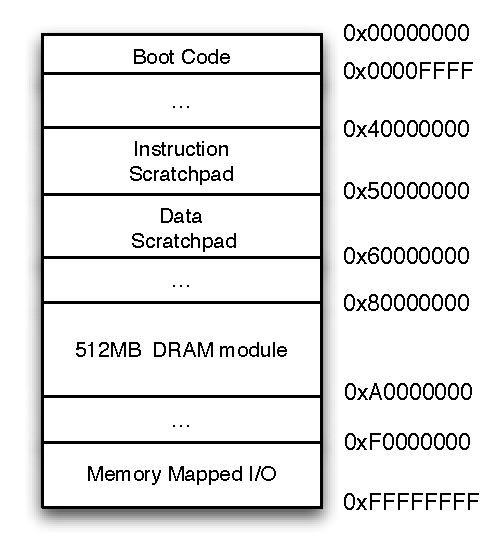
\includegraphics[scale=.65]{figs/ptarm_memory_layout}
  \end{center}
  \vspace{-20pt}
  \caption{Memory Layout of PTARM}
  \label{fig:ptarm_memory_layout}
  \vspace{-10pt}
\end{wrapfigure} 
The memory hierarchy of PTARM is exposed to the programmer, as discussed in section~\ref{section:memory_system}.
It is composed of a boot ROM (read only memory), instruction and data scratchpads, the predictable DRAM controller, and a memory mapped I/O region, all occupying separate address spaces.
Figure~\ref{fig:ptarm_memory_layout} shows the address regions occupied by each memory type.  

\subsection{Boot ROM}
The boot ROM \todo{mention boot code size} contains the reset instructions and exception vector table that stores entries for handling different exceptions that occur in the pipeline.
It also contains shared exception handlers and initialization code. 
The instructions store on the boot ROM cannot be modified at run-time, hence the read-only memory name. 
However, a dedicated region in the boot ROM stores a table for user-registered exception handlers, these entries can be modified prorammatically. 
We use this region to allow users to register timer expire exception handlers.
  
\subsection{Scratchpads}  
The instruction and data scratchpad \todo{size?} can be partitioned into private regions for each thread, or shared by all threads.
If PTARM is used in embedded security application, such as running encryption algorithms on it, then the partitioning the scratchpads into private regions might be desired. 
In chapter~\ref{chapter:app} we will discuss the security implications and how a Precision Timed Machine can defend against side-channel attacks.
On the other hand, sharing the scratchpad could provide flexibility on the allocation of scratchpads between hardware threads.
More space could be allocated to hardware threads running more memory intensive tasks while less could be allocated to the other hardware threads~\todo{cite scratchpad allocation paper}.
%The shared memory space in our system between hardware threads is also allocated on the data scratchpad, because the DRAM controller contains privatized bank resources, and does not allow
%FIXME: separate region for shared scratchpad space?
Both the boot ROM and scratchpads are synthesized to dual-ported block RAMs on the FPGA, and provide deterministic single cycle access latencies.

\subsection{DRAM}
\label{sec:ptarm_dram_integration}
\begin{wrapfigure}{r}{0.5\textwidth}
  \vspace{-20pt}
  \begin{center}
  	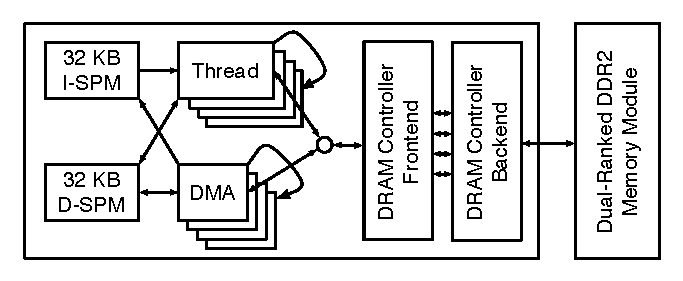
\includegraphics[scale=.6]{figs/pret-integration}
  \end{center}
    \vspace{-20pt}
  \caption{\small{Integration of PTARM core with DMA units, PRET memory controller and dual-ranked DIMM~\cite{ReinekeLiuPatelKimLee11_PRETDRAMControllerBankPrivatizationForPredictability}.}}
\label{fig:pretintegration}
  \vspace{-10pt}
\end{wrapfigure}
All access to the DRAM goes through the predictable DRAM controller described in section~\ref{sec:pret_dram_controller}.
The DRAM controller privatizes the DRAM banks into four resources, which we assign to each thread in our pipeline. 
This removes bank access conflicts and gives us predictable memory access latencies to the DRAM.
The pipeline interacts with the frontend of the DRAM controller, which routes requests to the right request buffer in the backend and manages the insertion of row-access refreshes to ensure the refresh constraint is met.   
In conventional memory architectures where the hierarchy is hidden, the processor interacts with DRAM indirectly by the filling and writing back of cache lines.
In our memory system, the processor can directly access the DRAM through load and store instructions to the distinct memory regions of the DRAM.
In addition, each hardware thread is also equipped with a direct memory access (DMA) unit, which can perform bulk transfers between the scratchpads and the DRAM.
Figure~\ref{fig:pretintegration} shows the integration of PTARM with the DMA units, memory controller and DRAM.  

\begin{wrapfigure}{r}{0.5\textwidth}
  \vspace{-25pt}
  \begin{center}
  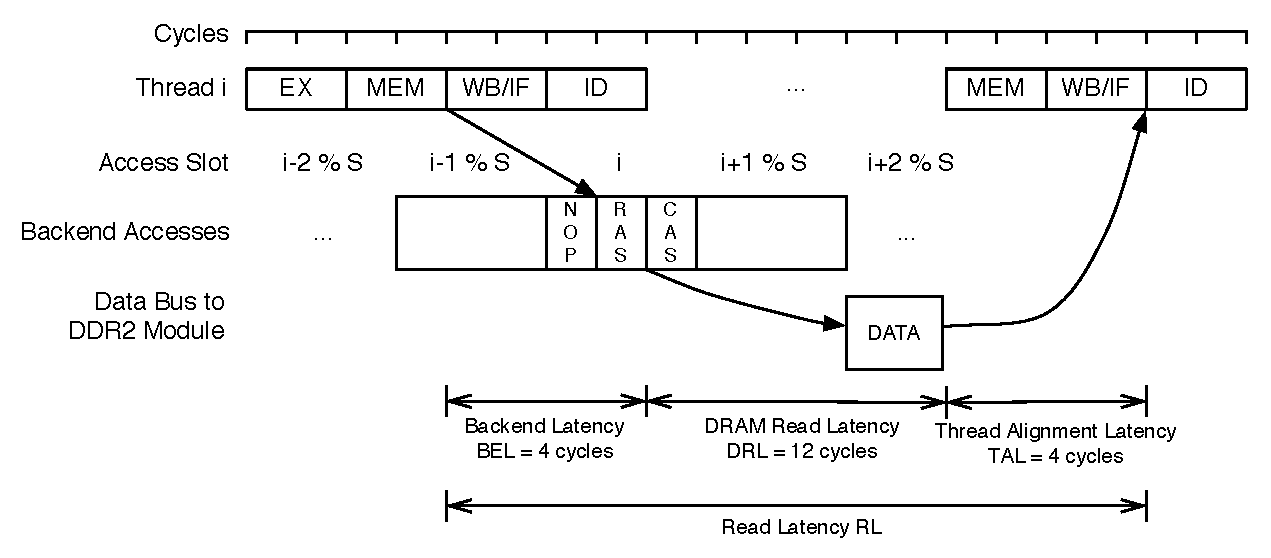
\includegraphics[scale=.38]{figs/readlatency}
  \end{center}
  \vspace{-20pt}
  \caption{\small{Example of a load operation by hardware thread $i$ in the thread-interleaved pipeline.}}
  \label{fig:readlatencyderivation}
\end{wrapfigure}
When DRAM is accessed through load (read) and store (write) instructions, the memory requests are issued directly from the memory stage of pipeline.
The request is received from the frontend of the memory controller, and placed in the correct request buffer. 
Depending on the alignment of the pipeline and the backend, it takes a varying number of cycles until the backend generates corresponding commands to be sent to the DRAM module.
After the read has been performed by the DRAM and has been put into the response buffer, again, depending on the alignment of the pipeline and the backend, it takes a varying number of cycles for the pipeline to reach the write-back stage of the corresponding hardware thread, which picks up the response. 
Figure~\ref{fig:readlatencyderivation}, illustrates the stages of the execution of an example read instruction in the pipeline.
In~\cite{ReinekeLiuPatelKimLee11_PRETDRAMControllerBankPrivatizationForPredictability} we derive the access latencies from the alignment and show that it is either 3 or 4 thread cycles.    
We leverage this misalignment of the pipeline and backend to hide the refresh latency from the front end. 
When a refresh is scheduled for the DRAM resource, if no memory request is in the request buffer, the refresh is serviced.
As mentioned in section~\ref{sec:pret_dram_controller}, if a refresh conflicts with a pipeline load or store, we push back the refresh till after the load or store. 
In this case, the pushed back refreshes become invisible:   
as the pipeline is waiting for the data to be returned and takes some time to reach the memory stage of the next instruction, it is not able to use successive access slots of the backend, and thus it is unable to observe the refresh at all.

Whenever a DMA transfer is initiated, the DMA unit uses the thread's request buffer slot to service DMA requests to/from the scratchpad. 
Thus, while a DMA transfer is initiated, the thread gives up access to the DRAM to the DMA unit.
During this time, the thread can continue to execute and access the scratchpad regions that is not being serviced by the DMA request. 
This is possible because scratchpads are dual-ported, allowing a DMA unit to access the scratchpads simultaneously as its corresponding hardware thread.
If at any point the thread tries to access the DRAM, it will be blocked until the DMA transfer completes.
Similarly, accesses to the region of the scratchpad being serviced by the DMA will also stall the hardware thread\footnote{This does not affect the execution of any of the other hardware threads.}.
%Since DMA units are not pipelined, there are no ``alignment losses'', so 
The DMA units can fully utilize the bandwidth provided by the backend because there are no alignment losses like the pipeline. 
When refreshes conflict with a DMA transfer, we push back the first refresh and schedule one at the end of the DMA transfer. 
This can be seen as shifting all refreshes, during the DMA transfer, back by $63$ slots or to the end of the transfer.
More sophisticated schemes would be possible, however, we believe their benefit would be slim.
With this scheme, refreshes scheduled within DMA transfers are predictable so the latency effects of the refresh can be easily analyzed, which we derive in~\cite{ReinekeLiuPatelKimLee11_PRETDRAMControllerBankPrivatizationForPredictability}.

\paragraph{Store Buffer}
\label{sec:ptarm_dram_store_buffer}
Stores are fundamentally different from loads in that a hardware thread does not have to wait until the store has been performed in memory.
By adding a single-place store buffer to the frontend, we can usually hide the store latency from the pipeline.
Using the store buffer, stores which are not preceded by other stores can be performed in a single thread cycle.
By \emph{thread cycle}, we denote the time it takes for an instruction to pass through the thread-interleaved pipeline.
Other stores may take two thread cycles to execute.
A bigger store buffer would be able to hide latencies of successive stores at the expense of increased complexity in timing analysis.

\subsection{Memory Mapped I/O}
Currently PTARM implements a primitive I/O bus for communicating with external inputs and outputs.
Access to the bus also occurs in the memory stage of the pipeline, by loading and storing to or from memory mapped I/O regions.
I/O devices snoop the address bus to determine whether the pipeline is communicating with the device or not.
The I/O bus is shared by all threads in the thread-interleaved pipeline, thus, in addition to address and data, a thread ID is also sent out. 
The I/O devices connected can choose to utilize the thread ID or not, depending on the functionality of the device. 
In section~\ref{sec:ptarm_vhdl_soft_core} below we will describe the I/O components that we have connected to our PTARM core.
Currently all I/O devices interface with the processor through memory mapped I/O registers that are read and written to in a single cycle, so no bus contention arises in our primitive bus implementation.

In order to ensure predictable access times to all I/O devices, a predictable bus architecture must be implemented.   
Several timing predictable bus architectures~\todo{cite} have been proposed, which can be used for this purpose. 
A predictable thread-aware I/O controller is also needed to ensure data from the I/O devices are read by the correct thread, and contention is properly managed.  
This is a future research challenge of PRET -- to predictably interface with various I/O devices.    

\section{Exception Handling}
\label{subsec:exception_handling_in_ptarm}
When exceptions occur in a single threaded pipeline, the whole pipeline must be flushed because of the control flow shift in the program. 
The existing instructions in the pipeline become invalid, and the pipeline overwrites the PC to jump to a specified exception handler. 
The ARM ISA specifies seven types of exceptions, and an exception vector table that points the PC to specified handler addresses when those exceptions occur. 
The exception vector table is stored in the BootROM in our implementation.
Exceptions can be triggered by external or internal events that occur in the pipeline, such as an toggling an external interrupt signal or using a software interrupt instruction to trigger the exception programmatically.
But no matter how the exceptions are generated, they must be handled predictably in the pipeline.
 
In the context of a thread interleaved pipeline, all threads are temporally isolated. 
Thus, an exception that occurs on one thread must not effect the execution of other threads in the pipeline.
In our pipeline, any exceptions or interrupts that occur during execution are latched at each stage and propagated down the pipeline with the instruction. 
An instruction flush signal is toggled to ensure that this instruction does not commit any state to memory or registers. 
The exception type is checked at the memory stage in the PC write logic before the next PC is committed.  
According to the exception type, the program state register bits are set, and the PC is redirected to the correct entry in the exception vector table. 
The current PC is passed on to the writeback stage to store in the link register (R14).
This provides a mechanism for the program return to the initial instruction where the exception occurs and re-execute it if desired, since the instruction did not complete its execution.
If the exception is generated from after a memory access and detected in the writeback stage, the PC forwarding path is used to fetch the exception vector entry for data memory exceptions. 
Note that it is up the each exception handler to save the register states and stack of the program.  

\begin{wrapfigure}{r}{0.5\textwidth}
  \vspace{-20pt}
  \begin{center}
    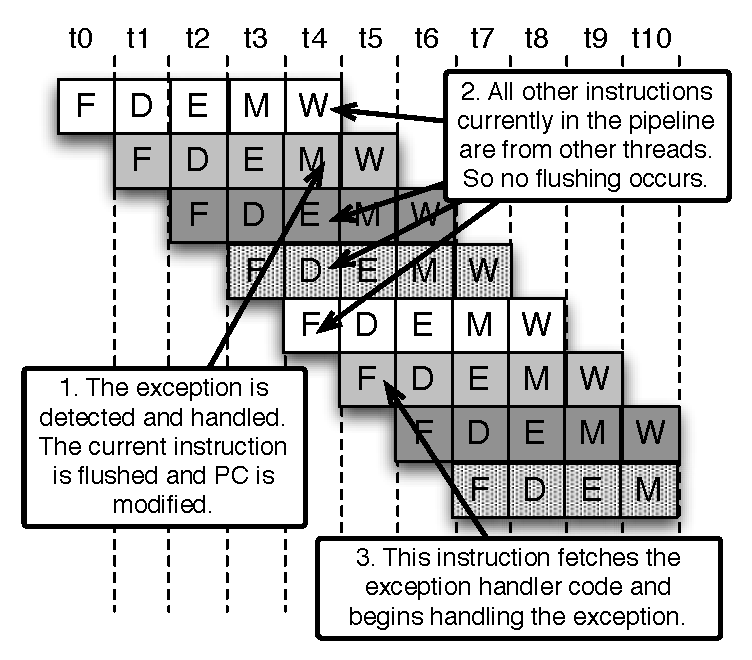
\includegraphics[scale=.65]{figs/exception_handling_pipeline}
  \end{center}
  \vspace{-20pt}
  \caption{Handling Exceptions in PTARM}
  \label{fig:exception_handling_pipeline}
  \vspace{-10pt}
\end{wrapfigure} 
None of the instructions that are executing in the pipeline are flushed when an exception occurs in our pipeline. 
As shown in figure~\ref{fig:exception_handling_pipeline}, the instructions that are executing in other pipeline stages all belong to other threads, so no flushing of the pipeline is required because no instruction was executed speculatively.
This simplifies the timing analysis of exceptions in our pipeline, as the timing behavior of other threads in the pipeline are unaffected.
For the thread which the exception occurs, the only overhead to handling the exception is that the current instruction does not complete its execution this thread cycle.  
The next thread cycle the pipeline will be handling the exception already, resulting in no additional stalls for the thread.

It is possible that an exception occurs during a memory access instruction that is waiting for the results from DRAM to complete. 
In this case, because the memory request is also sent to the DRAM controller, and possible already being serviced by the DRAM, we cannot cancel the memory request abruptly.
In the case that the interrupted instruction was a load, we can simply disregard the results of the load, but if the instruction was a store, we cannot cancel the store request that is writing data to the memory.
So it is up to the programmer to disable interrupts before writing to critical memory locations that require a consistent program state.
By interrupting an instruction that is waiting on memory access to complete, we also potentially complicate the interaction with our DRAM controller.
The DRAM controller can only service one request from each thread at a time for predictable performance\todo{elaborate on this?}.
This normally is not an issue because our pipeline does not reorder instructions or speculatively execute while there are outstanding memory requests, but the pipeline waits until the request is finished before continuing execution.
However, if a memory instruction is interrupted, the pipeline flushes the current instruction and continues execution of the exception handler in the Boot ROM.
If at this point, the exception handler contains a memory request instruction to the DRAM, a memory request would be issued to the DRAM controller that is still servicing the previous request prior to the exception from this thread.
The current memory request in this case would need to wait until the previous ``canceled'' memory request to complete its service by the DRAM before it can begin being serviced.
This creates timing variability to the load instructions because the execution time of load instructions would be different depending on whether an exception just occurred or not.
Because this situation can only occur in the exception handler, because it contains the instructions executed right after an exception, so we leave it to the compiler to ensure that the first few instructions in the exception handler code does not access the DRAM memory region.
In PTARM, the compiler simply needs to ensure that the first three instructions executed from an exception handler are not instructions that access the DRAM.

Currently PTARM does not implement an external interrupt controller to handle external interrupts. 
But when implementing such an interrupt controller, each thread should be able to register specific external interrupts that it handles.
For example, we might have a hard real-time task that is executing on one thread, while another thread without timing constraints is executing on another thread waiting for an interrupt to signal the completion of a UART transfer.
In this case the thread running the hard real-time task should not be effected even if it is in execution when the interrupt occurs.
Only the specific thread handling the UART transfers should be interrupt by this interrupt.  
So we envision an interrupt controller that allows each thread to register specific interrupts that it handles, without affecting other threads in the pipeline.  
%FIXME: Compare to XMOS style handling of interrupts?

\section{Instruction Implementations}
\label{sec:ptarm_instructions}
In this section we go into more details on how each instruction type is implemented and how each hardware block in the pipeline shown in figure~\ref{fig:ptarm_pipeline_five_stage}. 
We will go through different instruction types and discuss the timing implications each instruction in our implementation.
%FIXME: Talk about the difference between thread cycle and regular processor cycle
We will summarize with a table with all instructions and the cycle count it takes to execute them.
   
\subsection{Data-Processing}
We begin by explaining how data-processing instructions are implemented.
These instructions are used to manipulate register values by executing register to register operations. 
Most data-processing instructions take two operands.
One operand is always a register value, the second operand is labeled the shifter operand. 
The shifter operand could be an immediate value or a register value, both which can be shifted to form the final operand that is fed into the ALU.
Figure~\ref{fig:data_processing_pipeline_implementation} explains how data-processing instructions are executed through the pipeline.

\begin{figure}
  \vspace{-20pt}
  \begin{center}
    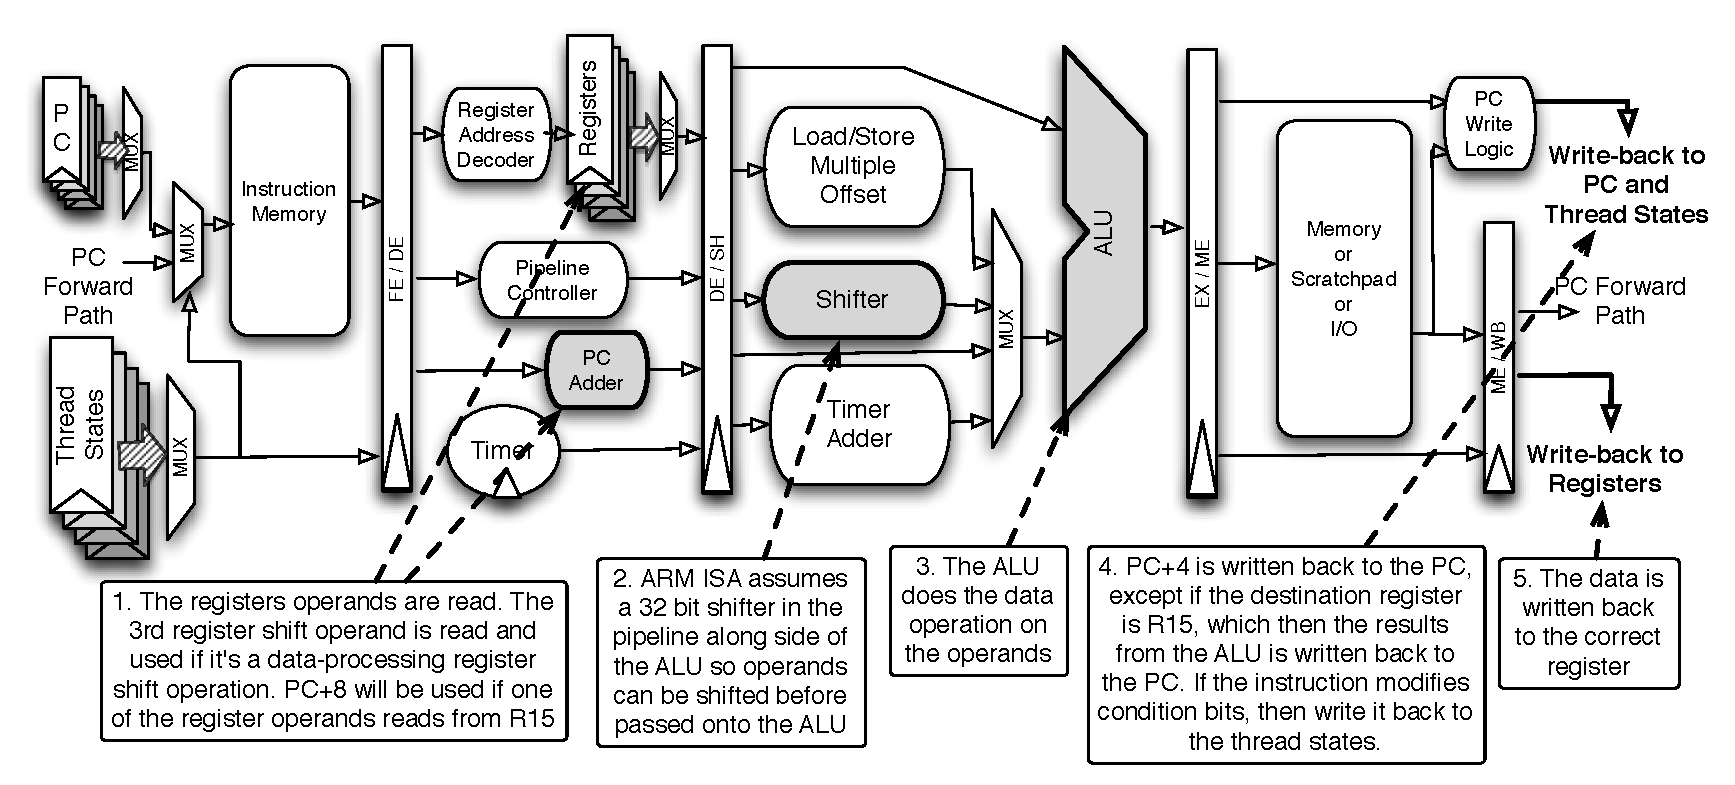
\includegraphics[scale=.54]{figs/data_processing_pipeline_implementation}
  \end{center}
  \vspace{-20pt}
  \caption{Data Processing Instruction Execution in the PTARM Pipeline}
  \label{fig:data_processing_pipeline_implementation}
\end{figure}

Because R15 is PC, so data-processing instructions that use R15 as an operand will read the value of PC+8 as the operand. 
Any instruction that uses R15 as the destination register will trigger a branch to the result of the computation.
As discussed earlier, our pipeline commits the next PC in the memory stage, so to trigger a branch from data-processing instructions simply means storing back the results from the ALU as the next PC.
In our thread-interleaved pipeline, when the next PC from the current thread is fetched, it will contain already contain the target address to branch to when we issue a data-processing instruction that writes to R15. 

Data processing instructions can also update the program condition code flags that are stored in the thread state. 
The condition code flags are used to predicate execution for ARM instructions, and consists of four bits: Zero (Z), Carry (C), Negative (N) and Overflow (V). 
The high four bits of each instruction forms a conditional field that is checked against the thread state condition code flags to determine whether or not the instruction is executed. 
The conditional execution for each instruction is checked in the pipeline controller. 
Data-processing instructions provide a mechanism to update the condition code flags according to the results of data operations.
The instructions that update the flags do not write any data back to the registers, they simply update the condition code flags.

All data-processing instructions only take one pass through the pipeline, even instructions that read from or write to R15, so all data-processing instructions take one thread cycle to execute. 
\subsection{Branch}
Branch instructions in the ARM can conditionally branch forward or backwards by up to 32MB.
There is no explicit conditional branch instruction in ARM.
Conditional branches are implemented using the ARM predicated instruction mechanism.
So the condition used to determine if a conditional branch is taken is simply the condition code flags in the thread state. 
Figure~\ref{fig:branch_pipeline_implementation} show how branch instructions are executed in the thread-interleaved pipeline.

\begin{figure}
  \vspace{-20pt}
  \begin{center}
    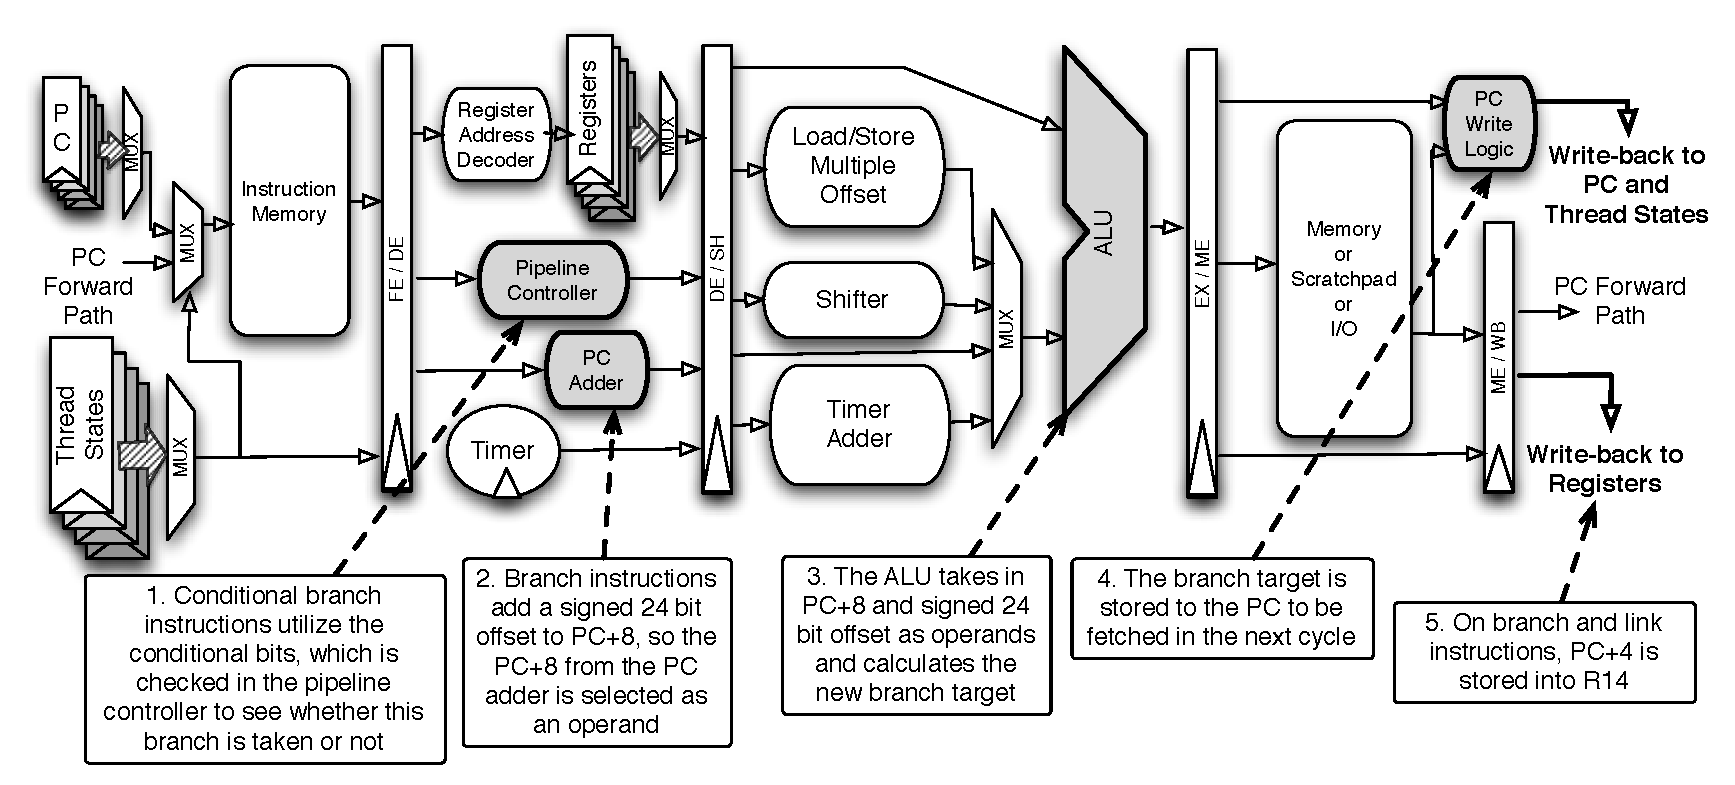
\includegraphics[scale=.54]{figs/branch_pipeline_implementation}
  \end{center}
  \vspace{-20pt}
  \caption{Branch Instruction Execution in the PTARM Pipeline}
  \label{fig:branch_pipeline_implementation}
\end{figure}

The branch instructions for the ARM ISA calculate the branch target address by adding a 24 bit signed offset, specified in the instruction, to the current PC incremented by 8. 
Thus, the PC adder, in addition to incrementing the PC by the conventional offset of 4, also increments the PC by 8, to be used as an operand for the ALU to calculate the target branch address.
Once the address is calculated, it is written back to its thread's next PC ready to be fetched. 
If the instruction is a branch and link ($bl$) instruction, PC+4 is propagated down the pipeline and written back to the link register (R14).   

All branch instructions, whether conditionally taken or not, all take only one thread cycle to execute.
But more importantly, the next instruction after the branch, whether it is a conditional branch or not, is not stalled or speculatively executed. 
The execution time of instructions from the same thread after the branch is not stalled nor affected by the branch instruction.  
The thread-interleaved pipeline simplified the implementation of the branch instruction and control hazard handling logic, as the pipeline will not need the results of the branch target address calculation the very next processor cycle.  
Instead, instructions from other threads will be fetched before the results of the branch is needed.

\subsection{Memory Instructions}
There are two type of memory instructions implemented in PTARM from the ARM ISA: Load/Store Register and Load/Store Multiple.
We discuss both type of memory instructions, and in particular, the interaction of the pipeline with the memory hierarchy presented earlier. 
We also present a special case when the load instruction loads to R15, which loads a branch target address from memory and triggers a branch.  
This slightly complicates our pipeline design, but we show that it does not affect the timing and execution of the instruction and subsequent instructions.
Currently load/store halfword doubleword is not implemented in PTARM, as they fall under the miscellaneous instructions category. 
These instructions can easily be implemented using the same principles described below without significant hardware additions.       
  
\subsubsection{Load/Store Register}
\label{sec:ptarm_instruction_ldstr}

Load instructions load data from the memory and writes them into the registers.
Store instructions store data from the registers into memory, thus store instructions utilize the extra register read port to read in the register value to be stored into memory.
The address used to access memory is formed by combining a base register and an offset value.
The offset value can be a 12 bit immediate supplied from the instruction, or a register operand that can be shifted.
The current load/store instructions can support word operations or byte operations.
Figure~\ref{fig:ldstr_pipeline_implementation} shows how the load/store instruction is executed in the pipeline.

\begin{figure}
  \vspace{-20pt}
  \begin{center}
    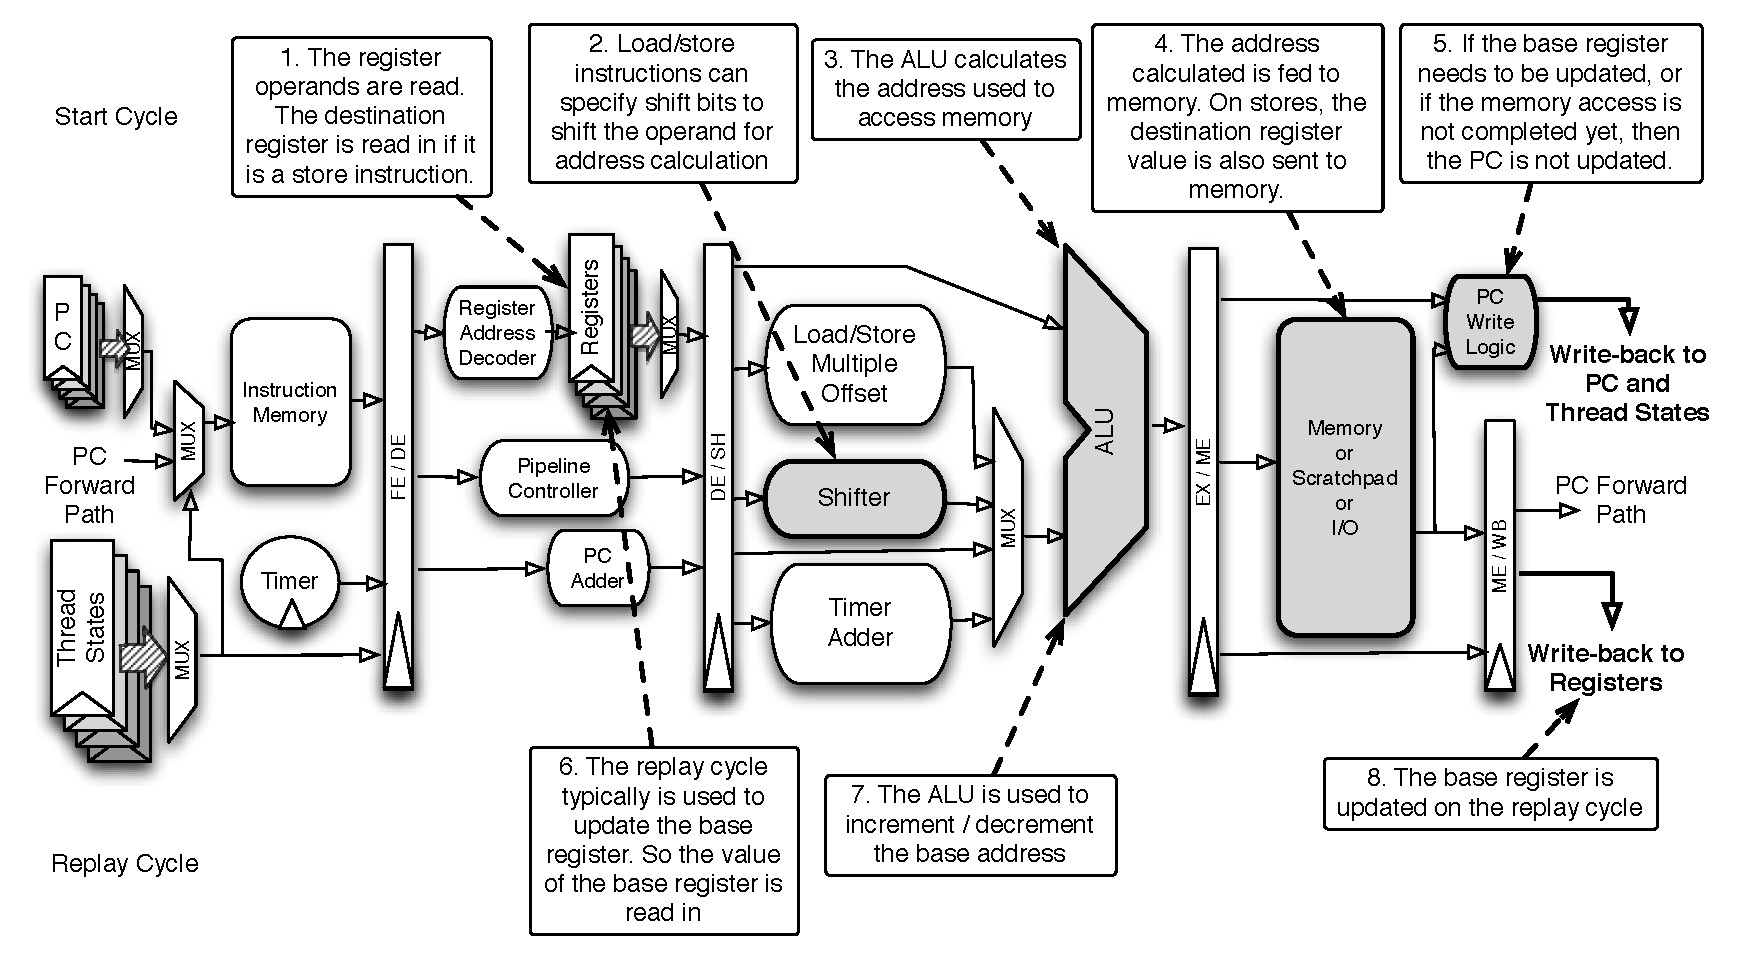
\includegraphics[scale=.54]{figs/ldstr_pipeline_implementation}
  \end{center}
  \vspace{-20pt}
  \caption{Load/Store Instruction Execution in the Ptarm Pipeline}
  \label{fig:ldstr_pipeline_implementation}
\end{figure}

All load and store instructions in ARM have the ability to update the base register after any memory operation. 
This compacts code that reads arrays, as a load or store instruction can access memory and updates the base register so the next memory access is done on the updated base register.
Different address modes differentiate how the base address register is updated. 
Pre-indexed addressing mode calculates the memory address by first using the value of the base register and offset, then updating the base register. 
Post-indexed addressing mode first updates the base register, then uses the updated base register value along with the offset to form the memory address.
Offset addressing mode simply calculates the address from the base register and offset, and does not update the base register. 
The base register could be either incremented or decremented. 
When pre and post-indexed addressing modes are used, memory operations require at least an additional thread cycle to complete.
Because the register file only contains one write port, we cannot simultaneously write back a load result from memory and the updated base register to the register file. 
Thus, we need to spend an extra pass through the pipeline to update the base register.

When the memory address is accessing the scratchpad memory region, memory operations can be completed in a single cycle, and the data is ready by the next (\emph{writeback}) stage to be written back to the registers.
However, if the memory read/write operation is accessing the memory region of the DRAM, the request must go through the DRAM memory controller to access the DRAM. 
%FIXME: update DRAM access latency
DRAM operations typically take three or four thread cycles to complete. 
As discussed in chapter~\ref{chapter:pret}, our thread-interleaved pipeline implementation does not dynamically switch threads in and out of execution when they are stalled waiting for memory access to complete. 
Thus, the when a memory instruction accesses the DRAM memory region, the same instruction is replayed by withholding the update for the next PC, until the data from DRAM arrives and is ready to be written back in the next stage.
For memory instructions accessing I/O regions, the access latency depends on the I/O accessed and the connection of the bus.  
As mentioned in section~\ref{sec:ptarm_memory}, the actual access time to I/O devices is device dependent, and a discussion of time-predictable buses is outside the scope of this thesis.
In the hardware implementation, for memory instructions that access the DRAM or I/O region, it is possible to update the base register earlier during the cycles where the instruction is waiting for access to complete.
However, the current PTARM implementation uses the same logic and datapath for all memory accesses (scratchpad, DRAM, I/O etc) to minimize hardware resources, so an additional cycle is used to update the base register for all memory accesses regardless of the address region they are accessing.

\subsubsection{Load/Store Multiple}
The load/store multiple instruction is used to load (store) a subset, or possibly all, of the general purpose registers from (to) memory.
This instruction is often used to compact code that pushes or pops registers from the program stack.
The list of registers that are used in this instruction is specified in the register list as a 16 bit field in the instruction.
The 0th bit of the bit field representing R0 and the 15th bit representing R15.
A base register supplies the base memory address that is loaded from or stored to, which then is sequentially incremented or decremented by 4 bytes for each register that is operated on. 
Figure~\ref{fig:ldstrm_pipeline_implementation} shows how the load/store multiple instruction is executed in the pipeline. 

\begin{figure}
  \vspace{-20pt}
  \begin{center}
    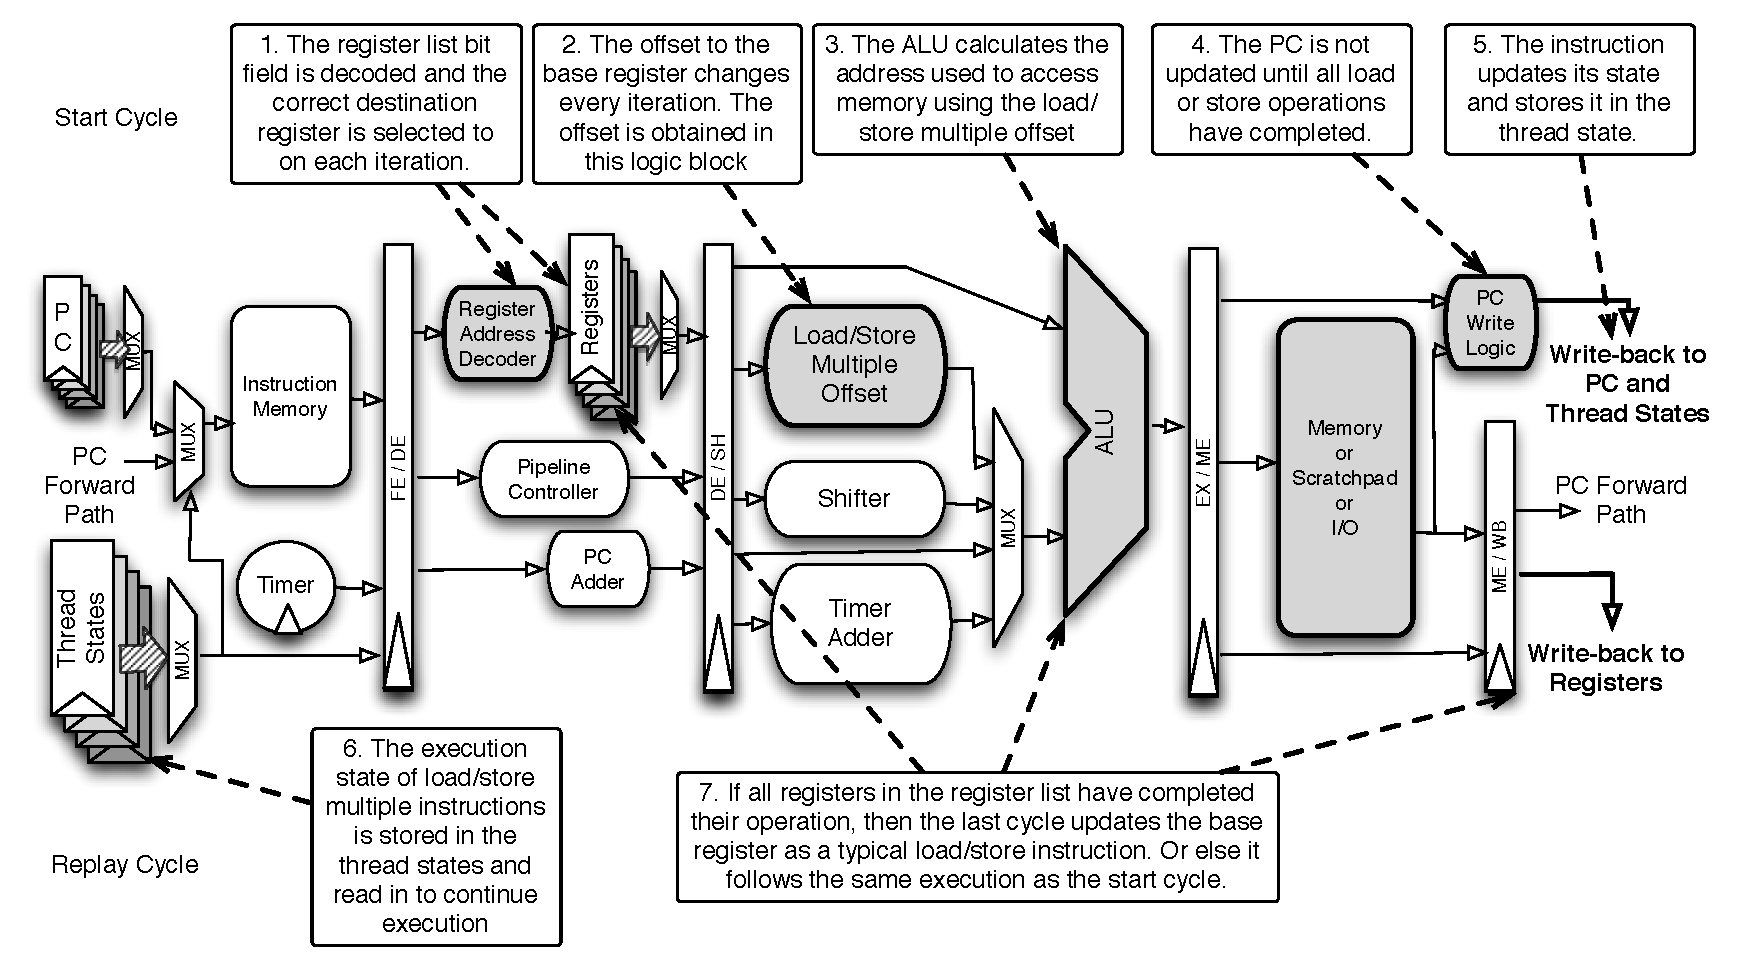
\includegraphics[scale=.54]{figs/ldstrm_pipeline_implementation}
  \end{center}
  \vspace{-20pt}
  \caption{Load/Store Multiple Instruction Execution in the PTARM Pipeline}
  \label{fig:ldstrm_pipeline_implementation}
\end{figure}

The load/store multiple instruction is inherently a multi-cycle instruction, because each thread cycle we can only write back one value to the register or store one value to memory. 
Thus, the execution state and remaining register list of the load/store multiple instruction is stored in thread state.
After the decoding the instruction, the remaining thread cycles load the register field from the thread state and clears it as registers are being operated on. 
The instruction completes when all registers have been operated on.
Each iteration the \emph{register address decoder} in the pipeline decodes the register list and determines the register being operated on.
For load multiple, this indicates the destination register that is written back to.
For store multiple, this indicates the register whose value will be stored to memory.
The \emph{load/store multiple offset} block is used to obtain the current memory address offset depending on how far we are in the execution of this instruction.
The offset is added to the base register to form the memory address fed into memory.

The execution time of this instruction depends on the number of registers specified in the register list and the memory region that is being accessed. 
For accesses to the scratchpad, each register load or store takes only a single cycle. 
However, if memory accesses are to the DRAM region, then register load/store will take multiple cycles.
It is also possible for the load/store multiple instruction to update the base register after all the register operations completes. 
Similar to the load/store register instruction, an additional thread cycle will be used to update the base register.
Although the execution time of this instruction seems to be dynamic depending on the number of registers specified in the register list, but the instruction binary will allow us to statically determine that number by parsing the bit field of the instruction.
Thus, the execution time of this instruction can still be statically analyzed.   

\subsubsection{Load to PC}    
When load/store operations load to the destination register R15, it triggers a branch in the pipeline.
This also holds true for the load multiple instruction if the 15th bit is set in the register list.
In our five stage pipeline, we commit the next PC in the memory stage so the next instruction fetch from the same thread can fetch the updated PC.
However, when the branch target address is loaded from memory, the address is not yet present in the memory stage to be committed, but only at the beginning of the writeback stage will it be present. 
Thus, we introduce a forwarding path that forwards the PC straight from the writeback stage to the fetch stage. 
Figure~\ref{fig:ld_to_pc_pipeline_implementation} shows how this is implemented in our pipeline.   
\begin{figure}
  \vspace{-20pt}
  \begin{center}
    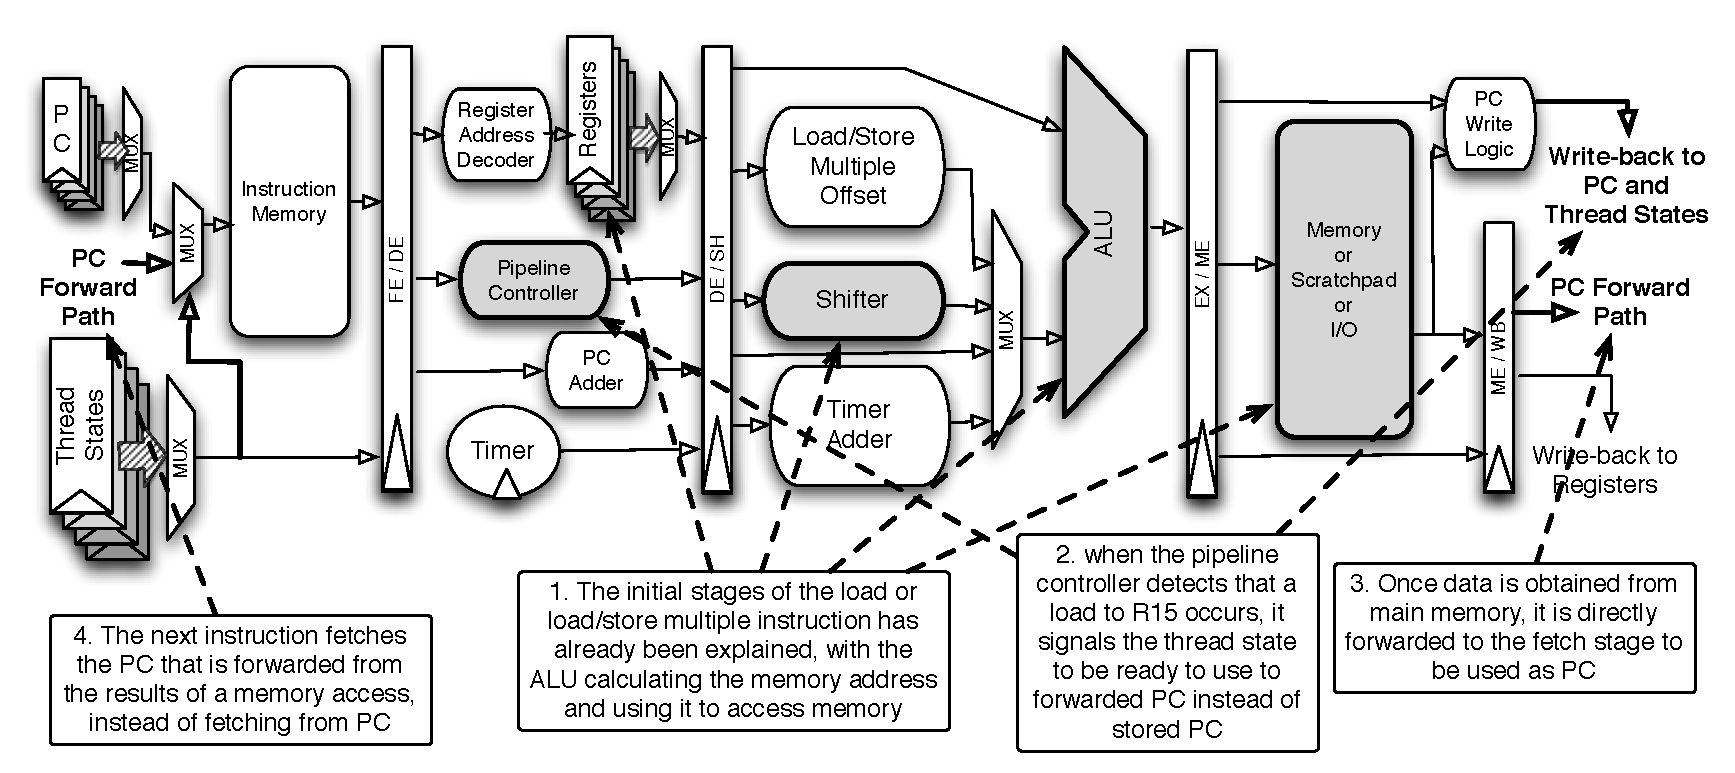
\includegraphics[scale=.54]{figs/ld_to_pc_pipeline_implementation}
  \end{center}
  \vspace{-20pt}
  \caption{Load to R15 Instruction Execution in the PTARM Pipeline}
  \label{fig:ld_to_pc_pipeline_implementation}
\end{figure}

An extra multiplexer is placed in the fetch stage before the instruction fetch to select the forward path.
When a load to R15 is detected, it will signal the thread state to use the forwarded PC on the next instruction fetch, instead of the one stored in next PC.
Because the data from memory will be ready at the beginning of the writeback stage, the correct branch target address will be selected and used.
We discussed in section~\ref{sec:pipeline_hazards} the timing implications of data-forwarding logic in the pipeline.
Those same principles are applied in this situation.
Although it seems the selection of PC is dynamic, but when forwarding occurs is actually static; this PC forwarding only and always occurs when instructions load from memory to R15.
This mechanism has no additional timing effects on any following instructions, as no stalls are needed to wait for the address to be ready. 
Even if the load to R15 instruction is accessing the DRAM region, the timing of this instruction does not deviate from a load instruction destined for other registers.
Although the target address will not be known until after the DRAM access completes, a load instruction that does not load to R15 also needs to wait until the DRAM access completes before the thread fetches the next instruction. 
So this extra forwarding mechanism does not cause load to R15 instructions to deviate from other load timing behaviors.

If the load to R15 instruction updates the base register, then the forwarding path is not used and not needed. 
The extra cycle used to update the base register will allow us to propagate the results from memory to be committed in the memory stage.
The timing behavior still conforms to a regular load to registers instruction. 

\subsection{Timing Instructions}
In section~\ref{sec:programming_models} we presented various instruction extensions to the ISA to bring timing semantics at the ISA level.
We will now present a primitive implementation of those instructions in PTARM.  
ARM provides extra instruction encoding slots to be used to implement instructions for co-processors attached to the core. 
In our case, we implement our timing instructions as part of co-processor 13.
We have already described the functionality and use case of the different timing instructions, table~\ref{table_deadline_insts} shows a summary of the instructions and their op codes.
All instructions have the assembly syntax ``\textbf{\textit{cdp, p13, $<$opcode$>$ rd, rn, rm, 0}}'', with $<$opcode$>$ differentiating the instruction type.
   
\begin{table}
\noindent\makebox[\textwidth]{%
\begin{tabular}{ | l | l | p{6cm} | }
  \hline                        
  Type & Opcode &  Functionality \\ \hline
  \textbf{\textit{get\_time}} & 8  & 
offset = (crm $<<$ 32) + crn; \newline
deadline = \textit{current\_time + offset}; \newline
crd = low32(deadline); \newline
crd+1 = high64(deadline); 
  \\ \hline 
  \textbf{\textit{delay\_until}} & 4 & 
deadline = (crm $<<$ 32) + crn; \newline
if ( \textit{current\_time} $<$ \textit{deadline} )  \newline
\hspace*{5 pt} stall\_thread(); 
 \\ \hline 
  \textbf{\textit{exception\_on\_expired}} & 2 &
offset = (crm $<<$ 32) + crn; \newline
register\_exception(offset);  
\\ \hline
  \textbf{\textit{deactivate\_exception}} & 3 &
deactivate\_exception();  
\\ \hline
\end{tabular}}
\caption{List of assembly deadline instructions}
\label{table_deadline_insts}
\end{table}

The timing instructions uses a master clock to obtain and compare deadlines.
PTARM implements the clock in the \emph{timer} block that is shown in figure~\ref{fig:ptarm_pipeline_five_stage}.   
Time is currently represented as an unsigned 64 bit value with nanoseconds as its units, and starts at zero when PTARM is reset. 
Unsigned 64 bits of nanoseconds can represent time up to approximately 584 years.
\todo{discuss timer implementation relative to different clock speeds. }
Each of the timing instructions operate on 64 bit values, which is stored in two 32 bit registers.
Because the deadlines are stored in general purpose registers, standard arithmetic instructions can be used to manipulate the values. 
However, PTARM does not current provide 64 bit arithmetic operations, so programmers must handle the overflow in software.

For each thread, the timer value is latched into the pipeline at the decode stage, which is where each thread's reference to time is.
Each thread operates on their own private deadlines, and are not affected by the timing instructions from other threads.
PTARM contains 4 hardware threads that are interleaved through the pipeline, so each hardware thread can only access the timer once every 4 processor clock cycles, the granularity of time observed by each thread.
We will discuss the timing implications of this in section~\ref{subsec:precision_timing_inst_ptarm}, in this section we merely present how they  are implemented in the pipeline.
	
\subsubsection{Get\_Time}    
The \emph{get\_time} instruction is used to obtain the current timer value and store it in two general purpose registers.
The \emph{get\_time} instruction also takes two optional source operands to calculate an offset to the current timer value. 
This allows the programmer to obtain the desired deadline time without additional arithmetic instructions.
Figure~\ref{fig:get_time_pipeline_implementation} shows how \emph{get\_time} is implemented in the PTARM pipeline. 
\begin{figure}
  \vspace{-20pt}
  \begin{center}
    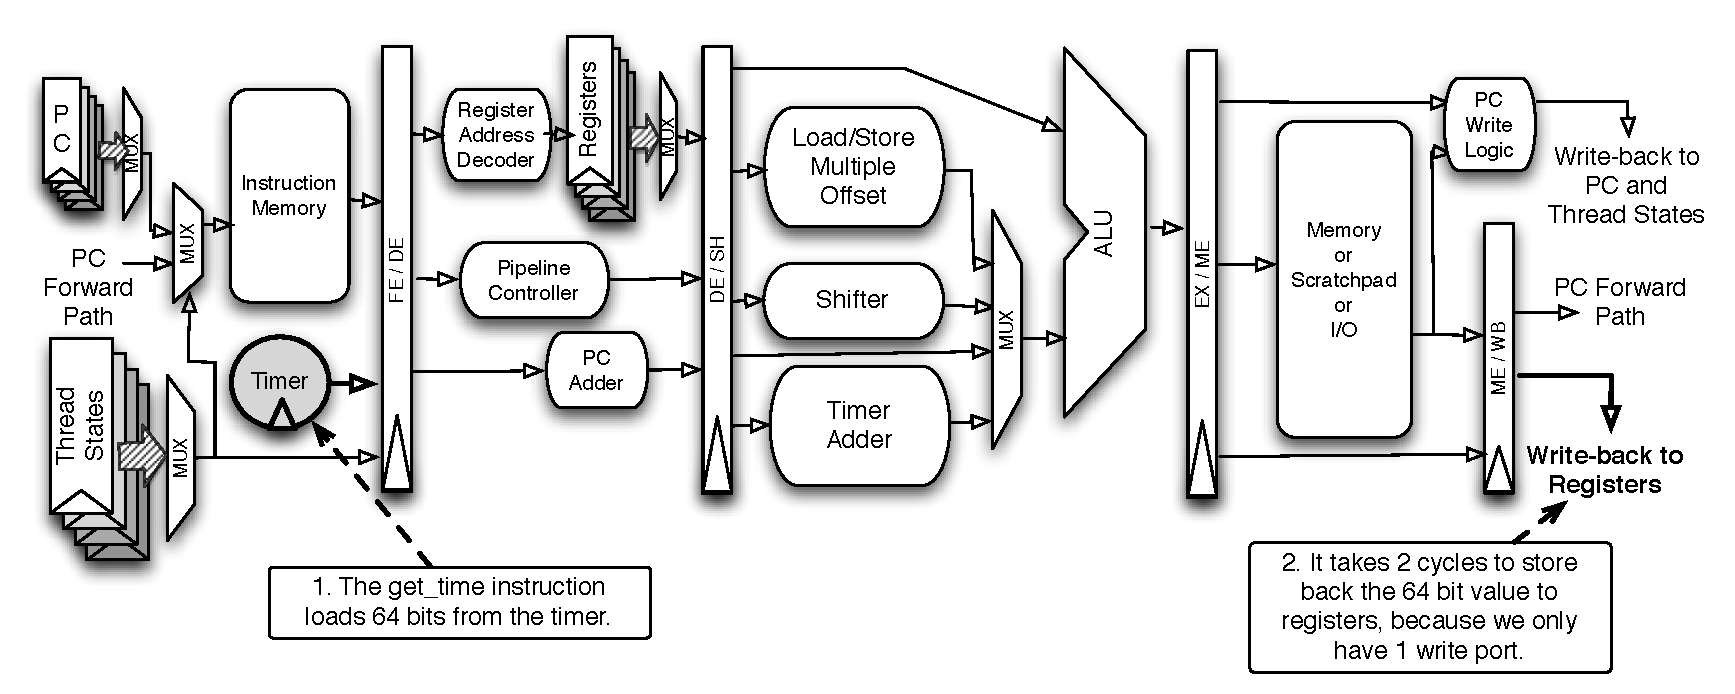
\includegraphics[scale=.54]{figs/get_time_pipeline_implementation}
  \end{center}
  \vspace{-20pt}
  \caption{Get\_Time Instruction Execution in the PTARM Pipeline}
  \label{fig:get_time_pipeline_implementation}
\end{figure}

The timer value and source registers are read in at the decode stage. 
The \emph{timer adder} adds the lower 32 bits of the timer value and source operand while the ALU computes the upper 32 bits taking into account the carry of the \emph{timer adder}.
Once the new deadline has been calculated, it is loaded back into the register file. 
Because our register file only contains one write port, so this instruction also takes two thread cycles to complete; each cycle writes back 32 bits of the new value. 
The calculated 64 bit deadline value is written to the destination register rd and rd+1, with rd storing the lower 32 bits and rd+1 storing the higher 32 bits. 
This instruction will not write to R15 (PC), and it will not cause a branch. 
If R14 or R15 is specified as rd, causing a potential write to R15, then this instruction will simply act as a NOP.

\todo{Talk about whether or not the time passed back adjusts for the latency of the instruction.}

\subsubsection{Delay\_Until}    
\emph{Delay\_until} is used to delay the thread until the a specified deadline has been reached.
It takes in 2 source operands which forms a 64 bit deadline value that is checked against the timer every thread cycle.
The 2 source operands are usually the results of a \emph{get\_time} instruction.  
As described in section~\ref{sec:programming_models}, the \emph{delay\_until} instruction can be used to specify a lower bound execution time for a code block.
This could be useful for synchronization between tasks or communicating with external devices.
Figure~\ref{fig:delay_until_pipeline_implementation} shows the implementation of the \emph{delay\_until} instruction in the PTARM pipeline.       
\begin{figure}
  \vspace{-20pt}
  \begin{center}
    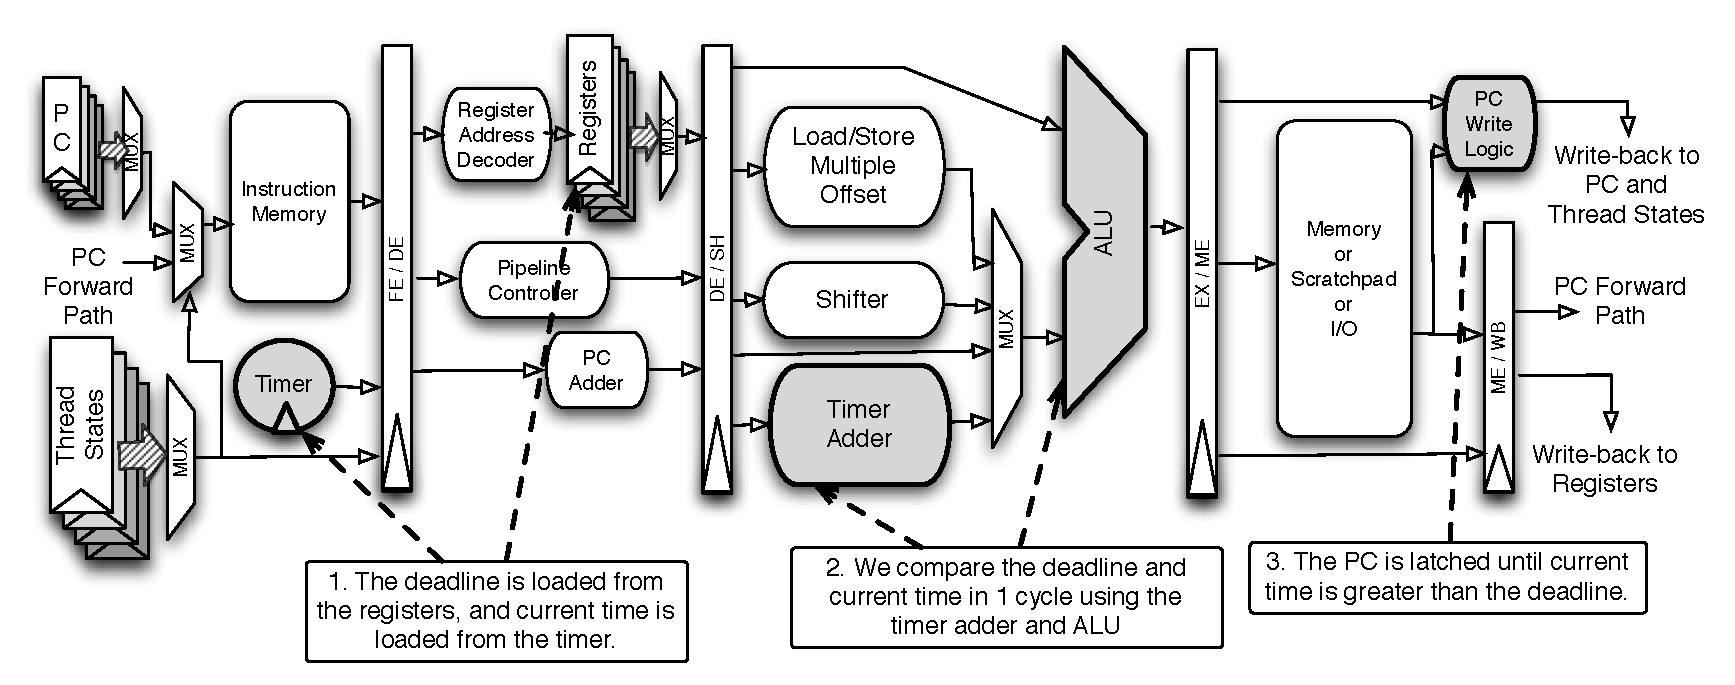
\includegraphics[scale=.54]{figs/delay_until_pipeline_implementation}
  \end{center}
  \vspace{-20pt}
  \caption{Delay\_Until Instruction Execution in the PTARM Pipeline}
  \label{fig:delay_until_pipeline_implementation}
\end{figure}

The implementation of the \emph{delay\_until} instruction is very straightforward, but highlights the reason the \emph{timer adder} is added into the pipeline.
The source operands and the timer value is latched at the decode stage, then compared using the \emph{timer adder} and ALU. 
The next PC is only updated if the timer value is greater than the deadline values passed in.  
Without the additional \emph{timer adder} in the pipeline, comparing 64 bits using our 32 bit ALU would take two thread cycles. 
This would decrease the precision of this instruction by a factor of two, because now we can only check the deadline against the timer every two thread cycles.
The added \emph{timer adder} allows \emph{delay\_until} to check the deadline every thread cycle, to ensure that no additional threads cycles have elapsed right after the deadline is reached. 

\subsubsection{Exception\_on\_Expire and Deactivate\_Exception}    
\emph{Exception\_on\_expire} and \emph{deactivate\_exception} provide a mechanism to actively check for missed code that runs longer than a specified deadline.  
\emph{Exception\_on\_expire} is used to register a deadline for immediate miss detection. 
\emph{Deactivate\_exception} is used to deactivate the active checking before the deadline expires.   
Unlike the \emph{delay\_until} instruction, which checks the deadline when the instruction is decoded, the deadlines registered with \emph{exception\_on\_expire} are checked in hardware in the background. 
A timer expired exception is triggered in the pipeline when a missed deadline is detected.
In section~\ref{sec:programming_models} we have outlines examples of how the instructions are used.

The actual execution of the \emph{exception\_on\_expire} and \emph{deactivate\_exception} instructions is straightforward.    
Within the \emph{timer} unit, there is one 64 bit deadline slot for each thread to register an actively checked deadline.
With four threads in PTARM, there are four slots in the \emph{timer} hardware. 
Whenever an \emph{exception\_on\_expire} instruction is executed, two source operands are read in and stored to the thread's corresponding deadline slot in the \emph{timer}. 
Every clock cycle of the timer, active deadlines are checked against the current timer value.
Once the current timer value surpasses one of the active deadlines, a timer expired exception for the particular thread is raised in the pipeline.
We add an entry to the existing ARM exception vector table to create this timer expired exception. 
The exception is handled the same as any other exception, as discussed in section~\ref{subsec:exception_handling_in_ptarm}, and is only handled by the thread that registered the deadline. 
The other threads in the pipeline remain temporally isolated from this exception.
The execution of a \emph{deactivate\_exception} instruction simply clears the deadline slot for the specific thread.

If threads need to simultaneously check for multiple deadlines, then the single deadline slot for the thread needs to be managed in software.
The software overhead involves managing a list of deadlines and ensuring that the earliest deadline is always being checked in the timer. 
It is possible to implement more than one deadline slot for each thread in the timer if more precise deadline checking is needed. 
However, this comes at the cost of additional hardware complexity in the timer, so currently in PTARM we simply have one deadline slot per thread, and use software mechanisms to manage multiple deadlines in a thread. 

\section{Realizations}
\subsection{PTARM VHDL Soft Core}
\label{sec:ptarm_vhdl_soft_core}
\begin{wrapfigure}{r}{0.5\textwidth}
  \vspace{-20pt}
  \begin{center}
    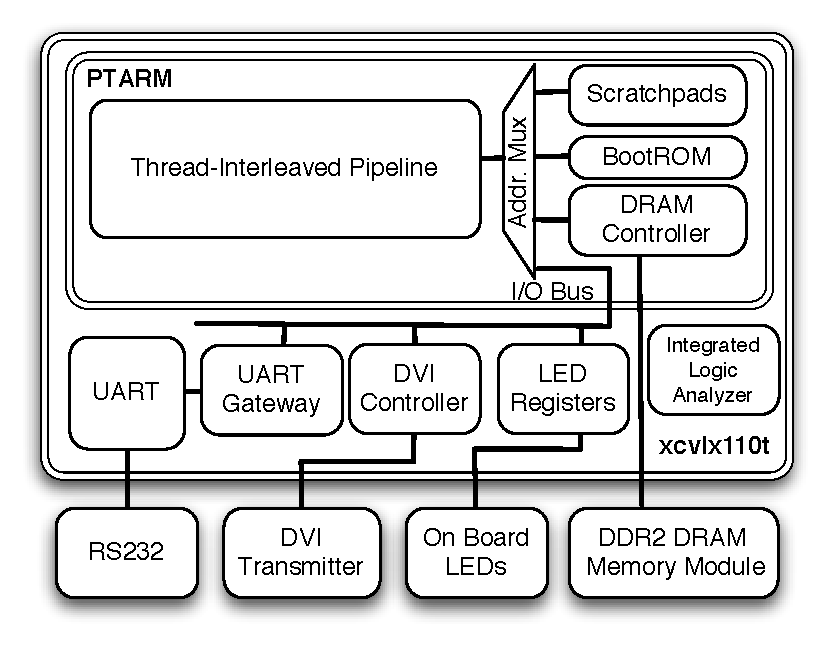
\includegraphics[scale=.6]{figs/ptarm_vhdl_high_level}
  \end{center}
  \vspace{-20pt}
  \caption{PTARM Block Level View}
  \label{fig:ptarm_vhdl_high_level}
  \vspace{-10pt}
\end{wrapfigure}   
The PTARM soft core is written in VHDL.
It includes the pipeline, scratchpad memories, predictable memory controller and connects to several I/O devices on the FPGA.
These include several LEDS, the UART, DVI controller and the DDRII DRAM.
All I/O devices are connected through the I/O bus, while the DDRII DRAM is connected directly to the DRAM controller.
Figure~\ref{fig:ptarm_vhdl_high_level} shows the high level block diagram of the PTARM soft core.

The LEDs are memory mapped and can be toggled by setting and clearing bits.
PTARM communicates to the UART through the UART gateway, which queues read and write requests from the core and relays it to the UART.
The default buffer size on the UART gateway is one.
The UART gateway status registers are mapped to memory I/O locations so programs can poll them to determine that status of the UART.  
Currently all read and write operations to the UART is done through blocking procedure calls. 
The UART runs at a baud rate of 115200 and can send and receive bytes.

The DVI controller is used to control the DVI input port on the FPGA, so a monitor can be connected.
\todo{look at documentation of the DVI controller, what mode we're using it.}
We demo a DVI controller application similar to the one presented in~\cite{ip2006processor}, where a vga controller is managed purely in software through the deadline instructions presented in the paper.
Here, we use the timing constructs presented in section~\ref{sec:programming_models} to control the sending out of vertical and horizontal sync signals in software.
As one hardware thread manages the sync signals, other hardware threads in our core can be used to calculate and draw to the screen buffer.  
Because hardware threads are temporally isolated, the timing of hardware sync signals are not affected by the operations on other hardware threads.  

We synthesized the core on a Virtex-5 lx110t FPGA to obtain the maximum clock frequency and resource usage. 
\todo{show area and clock speed on FPGA}  
We current clock PTARM at $100MHz$ and the memory controller at $200MHz$. 
All VHDL source code, software code samples, and instruction manual can be downloaded from http://chess.eecs.berkeley.edu/pret.   

\subsection{PTARM Simulator}
\label{sec:ptarm_sim}
Along with the VHDL soft core, we also developed a C++ cycle accurate software simulator of our architecture.
The simulator is meant for architectural exploration, and provides better debugging for software written for PTARM.  
The C++ simulator models the pipeline and memory hierarchy, including the predictable DRAM controller.  

The simulator provides a framework that allows us to do more architectural exploration and observe the behavior.
For example, the DMA units for each thread mentioned in section~\ref{sec:ptarm_dram_integration} that 
provide threads with the ability to transfer contents from the DRAM to the scratchpads in the background is currently only implemented on the simulator. 
The simulator allows us to quickly test out different software behaviors and verify our assumptions. 
The simulator and corresponding documentation can be downloaded from http://chess.eecs.berkeley.edu/pret. 

\todo{present benchmark numbers on the simulator and compare to others}

\section{Timing Analysis on PTARM}
\label{sec:wcet}
\label{subsec:precision_timing_inst_ptarm}

%mention that a full scaled worst case execution time analysis is beyond the scope of this thesis.
%but do a brief summary on how it's done, cite wilhelm's group's research summary
Worst-case execution time (WCET) analysis is a combined analysis of the control paths that the software might exhibit, and the time it takes to execute those paths on the underlying architecture. 
A plethora of research has been done on the software analysis of control paths. 
Wilhelm et al.~\cite{wilhelm-survey-paper} presented a survey of tools and techniques available for worst-case path enumeration and loop analysis etc.
However, the precision of the WCET analysis of those techniques ultimately depend on the underlying architecture implementation~\cite{Heckmann2003processor}.
Architectures that exhibit wildly unpredictable execution times will result in overly conservative WCET analysis, even if the software structure is simple. 
Designed as a predictable architecture, the instructions of PTARM all exhibit deterministic timing behaviors, allowing a more precise WCET as software analysis progresses. 
In section~\ref{sec:ptarm_instructions} we discussed the implementation of each instruction and explained the execution time of each instruction type.
Table~\ref{table:ptarm_instruction_timing} summarizes the execution time each instruction takes in terms of \emph{thread cycles}. 

\begin{table}[h]
\noindent\makebox[\textwidth]{%
\begin{smalltabular}{ | p{4cm} | c || p{9cm} | }
  \hline                        
  \textbf{Instruction Type} & \textbf{Thread Cycles} & \textbf{Notes}    \\ \hline
  Data Processing  & 1 & \multirow{2}{9cm}{ ${\ast}$: an additional cycle is added if pre or post-index offset is used in the address mode.}  \\ \cline{1-2} 
  Branch  & 1 &  \\ \cline{1-2}
  Load/Store (SPM)  & 1$^{\ast}$ &  \multirow{4}{9cm}{ ${\phi}$: the dram latency is 3 or 4 thread cycles depending on the alignment of the pipeline and the dram controller backend, as described in section~\ref{sec:ptarm_dram_integration}. For conservative estimates, 4 thread cycles is used. } \\ \cline{1-2} 
  Load/Store (BootROM)  & 1$^{\ast}$ & \\ \cline{1-2}  
  Load/Store (DRAM) & 4$^{\phi \dagger \ast}$ & \\ \cline{1-2}
  Load/Store Multiple & $N_{reg} \times L_{mem}$ $^{\Delta \ast}$ &  \\  \cline{1-2}
  Software Interrupt (SWI) & 1 & \multirow{4}{9cm}{ ${\dagger}$: a single store buffer is implemented, as described in section~\ref{sec:ptarm_dram_store_buffer}, so non-consecutive stores take only 1 thread cycle, while consecutive stores require the full dram latency of 3 or 4.}\\    \cline{1-2}
  get\_time  & 2 &  \\ \cline{1-2}
  delay\_until  & 1 $^{\sigma}$ & \\    \cline{1-2}
  exception\_on\_expire  & 1  &    \\   \cline{1-2}
  deactivate\_exception & 1 &  \multirow{2}{9cm}{ ${\Delta}$: $N_{reg}$ is number of registers specified in the instruction. $L_{mem}$ is the latency of the memory region operated on.} \\  \cline{1-2}
  \multicolumn{2}{|c|}{} &  \\ \cline{1-2}
  \multicolumn{2}{|c|}{} &   \multirow{2}{9cm}{${\sigma}$: denotes the minimum execution time. Actual execution time depends on the system clock and the specified deadline.} \\ \cline{1-2}
  \multicolumn{2}{|c|}{} &\\ \hline
\end{smalltabular}}
\caption{Timing properties of PTARM instructions \todo{change this table}}
\label{table:ptarm_instruction_timing}
\end{table}

A \emph{Thread cycle} is the unit used to represent execution time on each thread.  
Timing analysis can be done separately for each hardware thread running on PTARM because the threads are temporally isolated; the execution time of each thread cannot be affected by other threads.
The thread-interleaved pipeline switches thread contexts every processor cycle in a predictable round robin fashion. 
Thus, each thread is fetched and executed in the pipeline every $N$ processor cycles, $N$ being the number of threads in the pipeline.
One \emph{Thread cycle} represents each time the thread enters in the pipeline, which is the thread's perceived notion of cycles.
The execution frequency of each thread ($F_{thread}$) is $F_{thread} = F_{processor}/N$, so each \emph{thread cycle} is $1/F_{thread}$ long. 
For example, our PTARM core is clocked at 100$MHz$ ($F_{processor} = 100 * 10^6$) and has 4 threads ($N=4$) , so each thread cycle is $1/((100 * 10^6)/4) = 40 * 10^{-9}$ secs, or 40 nanoseconds long.
The length of the \emph{thread cycle} will not change because of the predictable thread-switching policy, making it a reliable unit of measurement for execution time.   


\subsection{Memory instructions}
Data-processing instructions typically have straightforward execution times on most architectures.
In our case, branch instructions also have very a predictable and straightforward execution, as the branch penalty is completely hidden within the thread interleaving.
The memory instructions in our architecture however can have several different latencies depending on addressing mode or region of access, as listed in table~\ref{table:ptarm_instruction_timing}.
For memory instructions that use pre or post-indexed addressing mode to update the base register, an additional cycle latency is needed to write back to the base register, as described in the instruction implementation in section~\ref{sec:ptarm_instruction_ldstr}.
But the addressing mode of load/store instructions can be determined statically, as it is part of the instruction encoding, so it does not affect the complexity or precision of execution time analysis. 

For load instructions, the exposed memory hierarchy allows us to clearly label and identify access latencies to different memory regions.
In execution time analysis, value analysis attempts to determine what memory addresses are accessed.     
In systems that use caches and hide the memory hierarchy, additional modeling of the cache state is still needed after the value analysis determines the potential memory addresses that are accessed.
However, with an exposed memory hierarchy with scratchpads, the precision of execution time analysis depends only on the value analysis. 
As soon as the memory address is determined, we can give a associate a precise memory access latency.
The worst-case DRAM latency of 4 thread cycles is derived from~\cite{ReinekeLiuPatelKimLee11_PRETDRAMControllerBankPrivatizationForPredictability}. 
This allows not only for a simpler timing analysis, but also a more accurate analysis.

For store instructions, the single store buffer as described in section~\ref{sec:ptarm_dram_store_buffer} can possibly hide the latency of store instructions if no other memory access instruction comes after it. 
Otherwise the store instruction will take the full memory access latency, depending on the memory access region of the store.
Timing analysis tools can mostly account for the store buffer by statically checking a few instructions ahead of the store instruction to see if there are memory accessing instructions.
The window of instructions that need to be checked is very narrow, so it should not really complicate the analysis.
If this is not possible, then conservatively, the full memory access latency should be used for each store, depending on the access region.

The execution time of load/store multiple instructions depend on the number of registers operated on, and the memory region it accesses. 
Because the register list is statically encoded in the instruction, the number of registers operated on can easily be statically determined.
Store multiple instructions do not benefit from the store buffer, so all accesses take the full memory access latency.
For each register that is operated on, the latency will depend on which memory region it accesses. 
The total execution time of the instruction will be the sum of the latencies for all register operations. 
If pre or post-indexed addressing mode is used, an extra cycle is added to update the base register, just as regular load/store instructions. 

\subsection{Timing instructions}
Even though the execution time of most timing instructions can be statically determined, they impact the execution time of the program in a very dynamic way.
For example, the execution of \exceptiononexpire\ and \deactivateexception\ only take one cycle, but when the \timerexpired\ exception is thrown, the execution time of the whole program is affected. 
To understand the timing effects of the timing instructions, we must understand the implementation effects on the precision of the timing instructions.
It is impossible for any hardware implementation to provide absolute precision of time, as we are limited by the precision of the digital synchronous circuits that discretize the notion of time. 
Although the timing extensions allow the manipulation of nanoseconds in software, with the thread-interleaved pipeline, the basic unit of time for each thread is one thread cycle, or 40 nanoseconds, in PTARM.
As a result, 40 nanoseconds is the shortest interval of time that is observable by each thread.
This can also be explained from the implementation of the pipeline.
Each thread only latches the timer value in the fetch stage, and the timestamp is propagated along the pipeline and associated with the instruction. 
Since there are four threads cycling in a round robin fashion, each thread latches the timer value only once every 4 processor cycles. 
With 100MHz clocking the pipeline in our implementation, 4 processor cycles is  equivalent to 40 nanoseconds. 

When setting deadlines, the execution time of the timing instructions must be taken into account. 
As explained in the implementation, each timing instruction latches the current platform time in the fetch stage.
That timestamp is used throughout instruction execution and associated as the current time.  
For example, the time value in the timestamp obtained from \gettime\ will contain the time before the execution of \gettime.
Since \gettime\ takes 2 thread cycles every execution, 80 nanoseconds will have elapsed when the timestamp is obtained from \gettime.
In the same way, \delayuntil\ latches the current platform time at the fetch stage each thread cycle, and compares with the input timestamp. 
\Delayuntil\ will delay program execution until the latched platform time is \emph{greater than or equal to} the input timestamp value.
So when \delayuntil\ completes its execution, the current platform time will be \emph{at least} 40 nanoseconds greater than the input timestamp specified, to account for the execution of \delayuntil. 

\begin{figure}[h]
  \begin{center}
    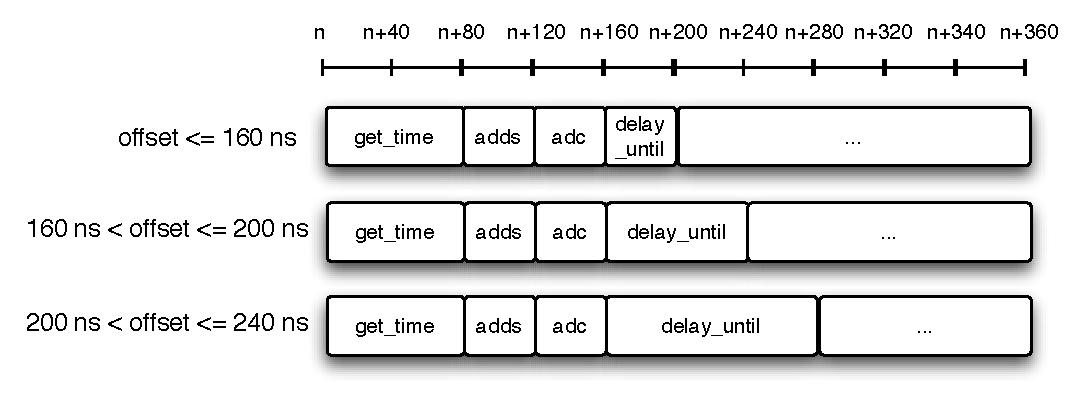
\includegraphics[scale=.7]{figs/delay_until_details}
  \end{center}
  \vspace{-3mm}
  \caption{Timing details of get\_time and delay\_until}
  \label{fig:delay_until_details}
\end{figure}

\todo{make figure for exception on expire!}

Figure~\ref{fig:delay_until_details} illustrates this effect by showing a timeline of execution for one thread on PTARM. 
The code segment starts executing at time $n$. 
The code only consists of \gettime, \delayuntil, and 2 add instructions used to add an offset to the timestamp obtained by \gettime.
For all 3 cases, the timestamp obtained by \gettime\ would contain the value $n$, even though the instruction after \gettime\ executes at $n+80$.
Taking into account the 2 thread cycles used to add the offset to the timestamp, if the offset is $\leq 160$, then the \delayuntil\ will simply serve as a NOP. 
This is because when \delayuntil\ is executed, it will latch $n+160$ for the platform time, and it will only delay program execution if the input timestamp is $> n+160$.
This is shown in the top case of the figure.
Notice that the instruction after \delayuntil\ executes at time $n+200$, which accounts for the 1 thread cycle it takes to execute \delayuntil.
Assuming \delayuntil\ does delay the program, in the worst-case, the instruction after \delayuntil\ executes $79 ns$ after the input timestamp. 
This can be observed if the offset is set to 161, which will result in the middle timeline shown in figure~\ref{fig:delay_until_details}.  
\Delayuntil\ will first latch the time $n+160$ to compare with the input timestamp of $n+161$. 
Because current platform time is less than input timestamp, \delayuntil\ will delay the execution of the program until the next cycle, when $n+200$ is latched to be checked against the input timestamp. 
At that point, \delayuntil\ will complete its execution, and the next instruction will execute at $n+240$.
This jitter results from the minimum observable time interval of $40 ns$ for each thread, causing \delayuntil\ to have an observable jitter of up to $40 ns$. 
\subsection{Timed Loop revisited}
\label{sec:timed_loop_revisited}
We give a concrete example of analysis of timing instructions on PTARM by deriving the \emph{offset} from the self compensating timed loop shown in section~\ref{sec:timed_loops}.
This timed loop detects whether the previous loop iteration missed its deadline. 
If it did, then the current iteration will execute a shorter version of the task in attempt to make up for the lost time, as shown in figure~\ref{fig:self_compensating_loop_timing}.  
\begin{figure}[h]
  \vspace{-3mm}
  \begin{center}
    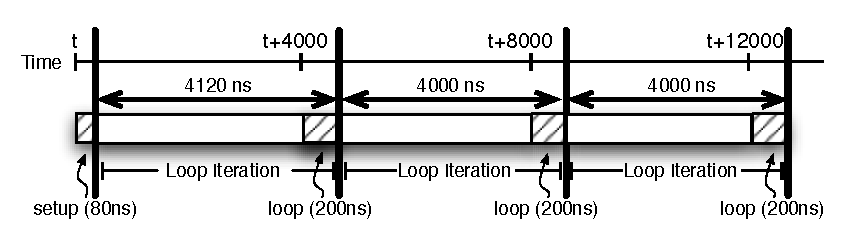
\includegraphics[scale=.7]{figs/self_compensating_loop_timing}
  \end{center}
  \vspace{-3mm}
  \caption{Execution of the self compensating timed loop}
  \label{fig:self_compensating_loop_timing}
\end{figure}
\vspace{-8mm}
\begin{lstlisting}[float=h, label=lst:timed_loop_compensate_revisit,caption=Timed loops with compensation revisited]
  cdp p13, 8, c2, c0, c0, 0  ; get_time, deadline timestamp stored in [c2, c3]
loop:
  cdp p13, 8, c4, c0, c0, 0  ; get_time, current timestamp stored in [c4, c5]
  subs r5, r5, #80           ; compensate for loop overhead and delay_until 
  sbc  r4, r4, #0            ; 

  subs r3, r3, r5            ; Check if previous iteration deadline is missed
  sbc  r2, r2, r4            ; 

  blmi task_short            ; execute shorter task if previous deadline mess 
  blpl task_normal           ; or else execute normal task 
  
  adds r3, r3, #4000         ; assuming the deadline is 4 us (4000 ns)
  adc r2, r2, #0             ; calculate the deadline timestamp for this iter.
  cdp p13, 4, c2, c2, c3, 0  ; delay_until
   
  b loop
\end{lstlisting}

\subsubsection{Obtaining the offset}

\begin{table}
\vspace{-5mm}
\begin{center}
\noindent\makebox[\textwidth]{%
\begin{smalltabular}{ | l | l | l r | }
  \hline
  \textbf{Time} & \textbf{TC} & \textbf{Instruction} & \textbf{Comment}\\ \hline \hline 
  t ns & n &  \textit{cdp p13, 8, c2, c0, c0, 0} & get\_time (deadline: t) \\  \hline
  \multicolumn{4}{|c|}{ -- -- Loop 1st iteration / No deadline miss -- -- } \\ \hline    
  t+80 ns & n+2 &  \textit{cdp p13, 8, c4, c0, c0, 0 } & get\_time, (current: t+80) \\
  t+160 ns & n+4 &  \textit{subs r5, r5, \#80} & (current -= 80)\\
  t+200 ns & n+5 &  \textit{sbc  r2, r2, r4} & (current: t)\\  
  t+240 ns & n+6 &  \textit{subs r3, r3, r5} & compare deadline (t) and current (t) \\
  t+280 ns & n+7 &  \textit{sbc  r2, r2, r4} & result is 0, clear cc[``n''] \\
  t+320 ns & n+8 &  \textit{blmi task\_short} & nop since cc[``n''] == 0\\
  t+360 ns & n+9 &   \textit{blpl task\_normal} & branch since cc[``n"] == 0\\  
    - ns & - &  \ldots & executing task\_normal \\  
  t+3800 ns & n+95 & \textit{adds r3, r3, \#4000} &  (deadline += 4000) \\
  t+3840 ns & n+96 & \textit{adc r2, r2, \#0} &  (deadline: t+4000) \\ 
  t+3880 ns & n+97 &  \textit{cdp p13, 4, c2, c2, c3, 0} & delay\_until, input timestamp is t+4000\\
  - ns & - & \ldots & delay\_until for 3 thread cycles\\  
  t+4040 ns & n+101 &  \textit{b loop} & jump back to loop \\ \hline
  \multicolumn{4}{|c|}{ -- -- Loop 2nd iteration / Deadline miss -- -- } \\ \hline    
  t+4080 ns & n+102 &  \textit{cdp p13, 8, c4, c0, c0, 0 } & get\_time, (current: t+4080)\\
  t+4160 ns & n+104 &  \textit{subs r5, r5, \#80} & (current -= 80)\\
  t+4200 ns & n+105 &  \textit{sbc  r2, r2, r4} & (current: t+4000)\\  
  t+4240 ns & n+106 &  \textit{subs r3, r3, r5} & compare deadline (t+4000) and current (t+4000)\\
  t+4280 ns & n+107 &  \textit{sbc  r2, r2, r4} & result is 0, clear cc[``n''] \\
  t+4320 ns & n+108 &  \textit{blmi task\_short} & nop since cc[``n''] == 0\\
  t+4360 ns & n+109 &   \textit{blpl task\_normal} & branch since cc[``n"] == 0\\  
  - ns & - &  \ldots & code for task\_normal \\  
  t+7960 ns & n+199 & \textit{adds r3, r3, \#4000} & (deadline += 4000) \\
  t+8000 ns & n+200 & \textit{adc r2, r2, \#0} & (deadline: t+8000) \\ 
  t+8040 ns & n+201 &  \textit{cdp p13, 4, c2, c2, c3, 0} & delay\_until, *no delay*\\
  t+8080 ns & n+202 &  \textit{b loop} & jump back to loop \\ \hline
  \multicolumn{4}{|c|}{ -- -- Loop 3rd iteration / Compensate with shorter task -- -- } \\ \hline    
  t+8120 ns & n+203 &  \textit{cdp p13, 8, c4, c0, c0, 0 } & get\_time, (current: t+8120)\\
  t+8200 ns & n+205 &  \textit{subs r3, r3, r5} & (current -= 80)\\
  t+8240 ns & n+206 &  \textit{sbc  r2, r2, r4} & (current: t+8040) \\
  t+8280 ns & n+207 &  \textit{subs r3, r3, r5} & compare deadline (t+8000) and current (t+8040)\\
  t+8320 ns & n+208 &  \textit{sbc  r2, r2, r4} & result is -40, set cc[``n''] \\
  t+8360 ns & n+209 &  \textit{blmi task\_short} & branch since cc[``n"] == 1 \\
  - ns & - &  \ldots & code for task\_short \\  
  t+10280 ns & n+257 &   \textit{blpl task\_normal} & nop since cc[``n''] == 1\\    
  t+10320 ns & n+258 & \textit{adds r3, r3, \#4000} & (deadline += 4000) \\
  t+10360 ns & n+259 & \textit{adc r2, r2, \#0} & (deadline: t+12000) \\ 
  t+10400 ns & n+260 &  \textit{cdp p13, 4, c2, c2, c3, 0} & delay\_until\\
  - ns & - &  \ldots & delay until time is t+12000 \\  
  t+12040 ns & n+301 &  \textit{b loop} & jump back to loop \\ \hline
   \multicolumn{4}{|c|}{ -- -- Loop 4th iteration / Execute normal task -- -- } \\ \hline    
  t+12080 ns & n+302 &  \textit{cdp p13, 8, c4, c0, c0, 0 } & get\_time, (current: t+12080)\\
  t+12160 ns & n+304 &  \textit{subs r3, r3, r5} & (current -= 80)\\
  t+12200 ns & n+305 &  \textit{sbc  r2, r2, r4} & (current: t+12000) \\
  t+12240 ns & n+306 &  \textit{subs r3, r3, r5} & compare deadline (t+12000) and current (t+12000)\\
  t+12280 ns & n+307 &  \textit{sbc  r2, r2, r4} & result is 0, clear cc[``n''] \\
  \hline 
\end{smalltabular}}
\end{center}
\vspace{-3mm}
\caption{Instruction execution trace of the self compensating timed loop\\ (TC = thread cycles)}
\label{table:timed-loop-compensate-timing}
\end{table}

\todo{state that we assume instruction is compiled to instruction scratchpad}
Listing~\ref{lst:timed_loop_compensate_revisit} shows the source code that is used to construct this timed loop. 
During the miss detection (lines 3 to 8), an additional \textit{offset} is used to compensate for the execution of \delayuntil\ and loop overhead.
Time elapses between the \delayuntil\ of the previous loop iteration (line 15), where the previous deadline timestamp is checked, and the \gettime\ used for miss detection (line 3) in the current iteration.
Without the offset compensation, the loop overhead will cause the miss detection to always detect a missed deadline.
This can be observed from table~\ref{table:timed-loop-compensate-timing}, where we show a sample execution trace of four iterations in this timed loop.  
Figure~\ref{fig:self_compensating_loop_timing} shows the timing behavior of these four iterations, where a missed deadline in the second iteration will cause the third iteration to compensate by executing the shorter version of the task.



In table~\ref{table:timed-loop-compensate-timing}, execution starts at time $t$.
As mentioned before, each thread cycle is $40ns$, which is reflect in the left most column that shows the progression of time.
We also show the thread cycle (TC) count, which starts at $n$ when execution begins.
The execution time of each instruction is according to table~\ref{table:ptarm_instruction_timing}.
In this code segment, we keep track of two timestamps each iteration. 
The \emph{deadline\_timestamp} keeps track of the loop deadlines, and is stored in registers r2 and r3.  
The \emph{current\_timestamp} is updated with \gettime\ in the beginning of each loop iteration to detect if the previous iteration missed its deadline.
It is stored in registers r4 and r5. 
The loop period is set to be $4 \mu s$, which is $4000 ns$ (100 thread cycles).
We add the loop period to the \emph{deadline\_timestamp} each loop iteration (lines 13 and 14 in the listing).  

\newcommand{\currentt}{\emph{current\_timestamp}}
\newcommand{\deadlinet}{\emph{deadline\_timestamp}}


The need for the \emph{offset} can be observed at the beginning of the second loop iteration.
At time $t+4080ns$, \gettime\ is called to initiate the miss detection sequence.
The previous \deadlinet\ is $t+4000$, which was met in the first iteration.  
However, \gettime\ updates the \currentt\ to $t+4080$, because the execution of \delayuntil\ and \emph{b loop} took 2 thread cycles combined. 
Thus, our miss detection accounts for this by subtracting the 2 thread cycles ($80ns$) overhead from \currentt\ before comparing it with \deadlinet.
In general, the overhead that needs to be account for is the time elapsed between the deadline checking \delayuntil\ instruction and the miss detection \gettime\ instruction.
Intuitively this is because we want to check whether the previous \delayuntil\ executed before the previous \deadlinet, so the \emph{offset} is used to calculate the time of execution of the previous \delayuntil.  

\subsubsection{Overhead of the self compensating timed loop}
In this self compensating timed loop, the loop period is set to $4000ns$, and regulated with the \delayuntil\ instruction.
However, the loop period includes the execution of the actual task along with the loop and timing control overhead.
The loop overhead in this example is only the branch instruction on line 17 in listing~\ref{lst:timed_loop_compensate_revisit}, which is 1 thread cycles (40 ns).
The overhead for timing control and self compensation consists of all the timing instructions, the arithmetic on the timestamps, and the 2 conditional branch instructions that determines which task to execute.
From table~\ref{table:timed-loop-compensate-timing} we can count a total overhead of 11 thread cycles including 1 \gettime\ (2 thread cycles), 1 \delayuntil\ (1 thread cycle), 6 arithmetic operations on the timestamps (6 thread cycles), and 2 conditional branch instructions (2 thread cycles).
Overall the timed loop contains an overhead of 12 thread cycles ($480ns$) , which means the executed tasks (both normal and short) have a timing requirement of 88 thread cycles ($3520ns$) in order for each loop iteration to meet its deadline.  
In the second loop iteration for our example, \emph{task\_normal} executed for 89 thread cycles, exactly one thread cycle over its timing requirement. 
As a result, the \delayuntil\ of the second loop iteration did not delay program execution, and the third iteration miss detection detects a missed deadline, and switches to execute \emph{task\_short}. 

\subsubsection{First loop iteration jitter}
The \emph{offset} previously derived is an overhead that is executed in every iteration of the loop.
In our code, the overhead only included the execution time of the \delayuntil\ and a branch, as we always unconditionally branch to the beginning of the loop. 
However, if the overhead was larger, for example, in a conditional loop structure, then it could introduce jitter for the first iteration.
An example is shown in figure~\ref{fig:setup_look_timing}, where we used an overhead of 200ns, instead of 80ns.
\begin{figure}[h]
  \vspace{-3mm}
  \begin{center}
    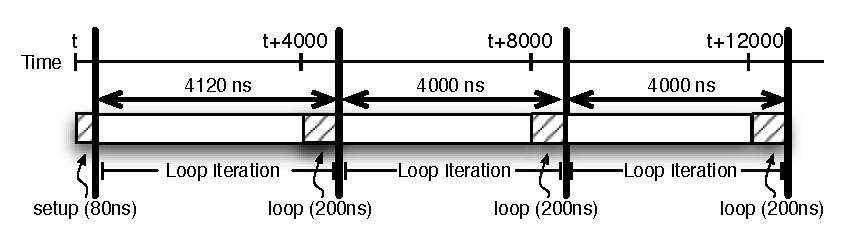
\includegraphics[scale=.9]{figs/setup_loop_timing}
  \end{center}
  \vspace{-3mm}
  \caption{Jitter caused by initial timed loop setup}
  \label{fig:setup_look_timing}
\end{figure}
We assume that the setup code remains the same with only one \gettime, and the \emph{offset} is adjusted to 200ns for the miss detection.
We also assume that the loop periond remains the same, 4000ns, and all loop iterations meet the loop period timing requirements. 
In this example, we see that the first iteration executes for 120ns longer than subsequent iterations.
The jitter for the first iteration is introduced by the execution time difference between the \emph{offset} and the setup code.  
Between the \delayuntil\ instructions, exactly 4000 ns elapses, because 4000 ns is added to the \deadlinet\ each loop iteration.   
The execution of the overhead is included within the 4000 ns, except for the first iteration. 
Instead, between the initial \deadlinet\ and the first \delayuntil, the only overhead that is observed is the execution of a \gettime\ instruction, which is 80 ns. 
Thus, the first iteration of the loop executes for an addition 120ns, which is the difference between the \emph{offset} and the execution time of the loop setup code.
This effect was not observed by the previous example because the \emph{offset} and the loop setup both took 80 ns.
As a result, for the previous example, each loop iteration takes exactly 4000 ns if all loop deadlines were met.   

\begin{lstlisting}[float=h, label=lst:timed_loop_compensate_adj,caption=Jitter adjusted timed loop ]
  mov r6, #0                 ; i = 0;
  mov r7, #0                 ; j = 0;
  
  cdp p13, 8, c2, c0, c0, 0  ; get_time, deadline timestamp stored in [c2, c3]
  subs r3, r3, #40           ; adjustment for first loop period 
  sbc  r2, r2, #0            ; deadline -= 40
loop:
  cdp p13, 8, c4, c0, c0, 0  ; get_time, current timestamp stored in [c4, c5]
  subs r5, r5, #200          ; compensate for loop overhead and delay_until 
  sbc  r4, r4, #0            ; 

  subs r3, r3, r5            ; Check if previous iteration deadline is missed
  sbc  r2, r2, r4            ; 

  blmi task_short            ; execute shorter task if previous deadline mess 
  blpl task_normal           ; or else execute normal task 
  
  adds r3, r3, #4000         ; assuming the deadline is 4 us (4000 ns)
  adc r2, r2, #0             ; calculate the deadline timestamp for this iter.
  cdp p13, 4, c2, c2, c3, 0  ; delay_until
	
  add r6, r6, #1             ; i += 1    
  add r7, r7, r6 LSL #1      ; j += i*2  
  cmp r7, #1000              ; 
  blt loop                   ; branch back if ( j < 10000 )
\end{lstlisting} 

\begin{figure}[h]
  \vspace{-3mm}
  \begin{center}
    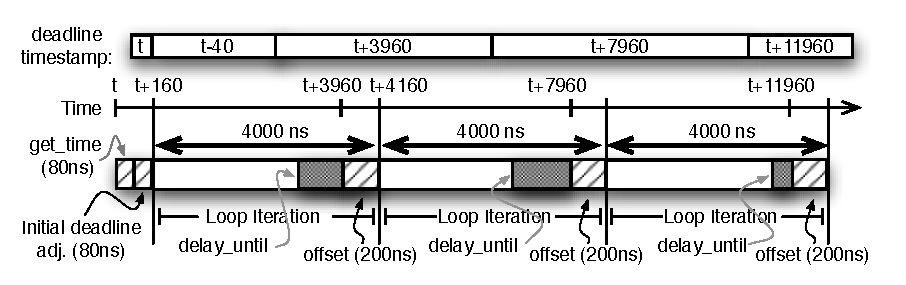
\includegraphics[scale=.9]{figs/setup_loop_timing_adj}
  \end{center}
  \vspace{-3mm}
  \caption{Adjusted timed loop setup}
  \label{fig:setup_look_timing_adj}
\end{figure}

This first iteration jitter can be accounted for by adjusting the initial \deadlinet\ in the loop setup code.
In listing~\ref{lst:timed_loop_compensate_adj} we show an example source code that adjusts for the additional overhead in the loop.
Lines 22 to 25 show the additional loop overhead that conditionally checks whether to branch back to the beginning of the loop.
The offset that we have to adjust for in this example is exactly 200ns, which includes the 4 instructions for the loop overhead and the \delayuntil. 
This offset is reflected on line 9.
Lines 4 to 6 show the loop setup code where we adjust for the execution time of the initial loop iteration, where 40 is subtracted from the initial \deadlinet\ obtained by the \gettime\ on line 4.
This value is obtained by the execution time difference of the overhead, which is $200ns$, and the setup code after \gettime, which is $160 ns$ (4 thread cycles).
We show the resulting timing behavior in figure~\ref{fig:setup_look_timing_adj}, where the first loop iteration is adjusted to 4000ns, the same as subsequent iterations.
By entering the loop with the \deadlinet\ value of $t-40$, we shift the \delayuntil\ deadlines for all loop iterations by 40 ns, allowing us to compensate for the first iteration jitter.   
Intuitively, we adjust the initial \deadlinet\ before entering the loop to create the illusion that the setup code and the loop overhead observed between each \delayuntil\ has the same execution time.
By doing so, the first loop iteration will observe the same loop period as all subsequent iterations. 

\subsection{Exceptions}
In section~\ref{subsec:exception_handling_in_ptarm} we described how exceptions are thrown in PTARM.
When an exception is triggered in one hardware thread, none of the other hardware threads are affected, as the pipeline is not flushed.
For the thread on which the exception occurred, only one thread cycle is lost, and the control flow jumps to the correct exception handler depending on the exception vector table.    
Here, we give a concrete example of the timing properties of exceptions on PTARM by showing how \exceptiononexpire\ and \deactivateexception\ trigger \timerexpired\ exceptions to handle missed deadlines immediately.
The code for the example is shown in listing~\ref{lst:exception-sample}.

\begin{lstlisting}[float=h, label=lst:exception-sample,caption=Sample code that triggers a \timerexpired\ exception ]
  mov  r3, #0x98              ; r3 = address of _timer_handler_loc 
  add  r4, pc, #32            ; r4 = addr of delay_handler
  str  r4, [r3]               ; register delay_handler
  
  cdp  p13, 8, c2, c0, c0, 0  ; get_time
  adds r3, #240
  adc  r2, #0
  cdp  p13, 2, c2, c2, c3, 0  ; exception_on_expire
  
  add  r5, r6, r6             ; arbitrary code block
  add  r7, r5, r6             ;
  
  cdp  p13, 5, c8, c2, c3, 0  ; deactivate_exception
  b end_program                       
  
delay_handler:
  mov pc, lr                  ; simply return
\end{lstlisting}

\newcommand{\delayhandler}{\emph{delay\_handler}}
\newcommand{\Delayhandler}{\emph{Delay\_handler}}
\newcommand{\timerhandlerloc}{\emph{\_timer\_handler\_loc}}

In this example, a \delayhandler\ is setup on lines 16 and 17 that simply returns when called.
\Delayhandler\ is registered as the exception handler for the \timerexpired\ exception, which happens on lines 1 to 3.
This is done by deriving the address of the \delayhandler\ on line 2, and storing it to the \timerhandlerloc.
The \timerhandlerloc\ is a reserved location that points to the address of the handler that is executed when the \timerexpired\ exception is thrown.
When a \timerexpired\ exception is thrown, the current address is saved and control flow jumps to the exception table entry for the \timerexpired\ exception.
This table entry redirects the execution to a \timerexpired\ exception setup code (shown in listing~\ref{lst:timer-expire-handler}) which calls the registered exception handler.
The setup code loads the address of \timerhandlerloc\ into a register, and jumps to the handler on line 7.
If the handler returns, lines 8 to 10 re-enable interrupts, and line 11 returns control to the original PC when the exception occurred.  
\begin{lstlisting}[float=h, label=lst:timer-expire-handler,caption=The \timerexpired\ exception setup code]
.text
.global _tmr_exp_setup;
_tmr_exp_setup:
    push  {r0, lr}                 ; push registers to stack
    ldr   r0, _timer_handler_loc   ; load address of timer expired exception handler
    mov   lr, pc                   ; get return address after calling handler    
    mov   pc, r0                   ; jump to exception handler
    
    mrs   r0, cpsr                 ; get CPSR 
    bic   r0, r0, #0x80            ; enable interrupts
    msr   cpsr, r0                 ; write to CPSR
    pop   {r0, pc}                 ; pop stack and return from exception

_timer_handler_loc: .word  0x00000000;
\end{lstlisting}

The execution trace of this example is shown in table~\ref{table:exception-expire-timing}.
\begin{table}[h]
\begin{center}
\noindent\makebox[\textwidth]{%
\begin{smalltabular}{ | c | c | l | l r | }
  \hline                        
  Time & TC & Address & Inst & Comment\\ \hline
  t ns & n & 0x40000000 & \textit{mov r3, \#0x98} & gets the \timerhandlerloc \\  
  t+40 ns & n+1 & 0x40000004 & \textit{add r4, pc, \#32} & get \delayhandler address \\
  t+80 ns & n+2 & 0x40000008 & \textit{str r4, [r3]} & register \delayhandler as timer expire handler\\
  t+120 ns & n+3 & 0x40000014 & \textit{cdp p13, 8, c2, c0, c0, 0} & get\_time (timestamp: t+120) \\
  t+200 ns & n+5 & 0x400000C & \textit{adds r3, \#240} & timestamp += 240 \\
  t+240 ns & n+6 & 0x40000010 & \textit{adc r2, \#0} & timestamp: t+360 \\
  t+280 ns & n+7 & 0x40000018 & \textit{cdp p13, 2, c2, c2, c3, 0} & exception\_on\_expire, input timestamp: t+360 \\
  t+320 ns & n+8 & 0x4000001C & \textit{add r5, r6, r6} & code block\\
  t+360 ns & n+9 & 0x40000020 & **throw exception** & timer expired, hardware exception thrown\\  
  t+400 ns & n+10 & 0x1C & \textit{b \_tmr\_exp\_setup } & branch to setup code \\  
  t+440 ns & n+11 & 0x78 & \textit{push \{r0, lr\}} & push registers to stack\\
  t+560 ns & n+14 & 0x7C & \textit{ldr   r0, \_timer\_handler\_loc} & load address of timer expired handler \\
  t+600 ns & n+15 & 0x80 & \textit{mov   lr, pc} & store return address after timer handler \\
  t+640 ns & n+16 & 0x84 & \textit{mov   pc, r0} & jump to handler (\delayhandler) \\
  t+680 ns & n+17 & 0x4000002C & \textit{mov   pc, lr} & \delayhandler\ code, return\\  
  t+720 ns & n+18 & 0x88 & \textit{mrs   r0, cpsr} & get CPSR\\
  t+760 ns & n+19 & 0x8C & \textit{bic   r0, r0, \#0x80} &  enable interrupts\\
  t+800 ns & n+20 & 0x90 & \textit{msr   cpsr, r0} &  write to CPSR\\
  t+840 ns & n+21 & 0x94 & \textit{pop   \{r0, pc\}} & pop stack and return from exception\\
  t+960 ns & n+24 & 0x40000020 & \textit{add r7, r5, r6} & re-execute instruction \\
  t+1000 ns & n+25 & 0x40000024 & \textit{cdp p13, 3, c2, c0, c1, 0} & \deactivateexception\ (does nothing) \\
  t+1040 ns & n+26 & 0x40000028 & \textit{b end\_program} & jump to end of program \\
  \hline 
\end{smalltabular}}
\end{center}
\caption{Exception\_on\_expire sample code timing details}
\label{table:exception-expire-timing}
\end{table}
Because execution jumps back and forth between the main code, the \timerexpired\ setup code, and the \delayhandler, so we show the address of the instructions to help follow which code segment is being executed.
The user code is compiled to start at 0x40000000, which is the instruction scratchpad space for hardware thread 0, which we assume this code is running on.
As described in section~\ref{sec:ptarm_memory}, the exception vector table and \timerexpired\ setup code are all compiled to the memory space of the boot ROM.
The \emph{str} instruction is storing to the \timerhandlerloc, which also resides in the boot ROM, so executes in one thread cycle.  
The deadline timestamp is set so the timer expired exception is thrown during the execution of the code block, which occurs at time $t+360$.
Although the address of execution at that time is 0x400000020, the instruction at that address does not complete, because the \timerexpired\ exception is thrown in that thread cycle.
That address is saved to the \emph{link register} (R14) in hardware when the exception is thrown.
The very next thread cycle, the exception vector entry for the \timerexpired\ entry (at address 0x1C) is executed. 
The entry forces a branch to the \timerexpired\ setup code, which executes to call the \delayhandler, the registered the exception handler.       
The \emph{push} and \emph{pop} instructions are load/store multiple instructions that load to the stack, which is located on the data scratchpad. 
These instructions update the base register, and are operating on 2 registers each, so they both take 3 thread cycles to execute.
In section~\ref{subsec:exception_handling_in_ptarm} we discussed the potential execution variability for memory operations if the instruction interrupted by the exception is a long latency memory operation to the DRAM. 
In order to maintain a deterministic execution time for all memory operations, the compiler ensures that the first four thread cycles (the DRAM access latency) after an exception is thrown does not access the DRAM. 
The exposed memory hierarchy with scratchpads allows us to statically compile the exception setup code and data stack, both accessed right after an exception is thrown, onto the scratchpad. 
This ensures that the DRAM is not accessed during the first four thread cycles after the exception is thrown.

The timing analysis of exceptions thus is straightforward in the PTARM architecture.
No flushing of the pipeline occurs, no other hardware threads are affected, and the hardware exception mechanism only has a one thread cycle hardware overhead.
Due to deterministic instruction execution time and exposed memory hierarchy, the \emph{response time} of hardware exceptions, which is the time elapsed between when the exception is thrown and when the user registered exception handler is executes, is deterministic and can be statically obtained. 
For the \timerexpired\ exception in PTARM, the response time is 8 thread cycles ($320ns$), which is reflected in table~\ref{table:exception-expire-timing}.



